\documentclass{article}
% Paquetes de idioma y codificación de caracteres
\usepackage[english,spanish]{babel}
\usepackage[utf8]{inputenc}
\usepackage[T1]{fontenc}

% Paquetes de escritura matemática
\usepackage{amsmath,amsfonts,amssymb,bm,mathtools}

% Márgenes y tamaño del folio
\usepackage[left=2cm,right=2cm,top=2cm,bottom=2cm,a4paper]{geometry} 

% \usepackage{multirow} %Múltiples filas
% \usepackage{graphicx} %Gráficos
% \usepackage{soul} %Subrayar
% \usepackage{fancybox} %Cajitas guays
% \usepackage{multicol}
% \usepackage{cancel}
% \usepackage{pdfpages} %Inserción PDF
% \usepackage{tabu}%Ahorra tener que estar usando $ todo el rato en tablas
% \usepackage{realboxes}
% \usepackage{titlesec} %spacing before and after section titles
% \usepackage{lipsum} %texto de ejemplo
% % \usepackage{natbib}
% \usepackage{babelbib}
% \usepackage{urlbst}
\usepackage{siunitx}

\usepackage{color}
\usepackage{enumitem}% http://ctan.org/pkg/enumitem 
\usepackage{bbold} %identitity matrix symbol ("double" one)
	
	
% Definición de comandos: 
\newcommand{\abs}[1]{\left\lvert#1\right\rvert} %valor absoluto/módulo
\newcommand{\norm}[1]{\left\lVert#1\right\rVert} %norma
\newcommand{\refer}[1]{$^{[\ref{#1}]}$} %Referencias en superíndice
\newcommand{\uni}[1]{\ \mathrm{#1}} %Unidades con separación de un 'en' y  sin cursiva
\newcommand{\dif}{\mathrm{d} } %diferencial con d en roman
\newcommand{\der}[2]{\frac{\mathrm{d}#1}{\mathrm{d}#2}} %derivada de #1 resp a #2
\newcommand{\derd}[2]{\frac{\mathrm{d}^2#1}{\mathrm{d}#2^2}} %derivada segunda de #1 resp a #2
\newcommand{\dert}[2]{\frac{\mathrm{d}^3#1}{\mathrm{d}#2^3}} %derivada tercera de #1 resp a #2
\newcommand{\parc}[2]{\frac{\partial#1}{\partial#2}} %derivada parcial de #1 resp a #2
\newcommand{\parcd}[2]{\frac{\partial^2#1}{\partial#2^2}} %derivada de #1 resp a #2
\newcommand{\curl}{\nabla\times} %curl operator
\newcommand{\rot}{\nabla\times}  %operador rotacional
\newcommand{\diver}{\nabla\cdot} %operador divergencia
\newcommand{\laplac}{\nabla^2}
\newcommand{\mean}[1]{\langle #1\rangle } %Media
\newcommand{\pe}[2]{\langle #1|#2\rangle } %Producto escalar
\newcommand{\bra}[1]{\left\langle#1\right|}  %bra
\newcommand{\ket}[1]{\left|#1\right\rangle} %ket
\newcommand{\braket}[2]{\left\langle#1\right|\left.#2\right\rangle} 
% \newcommand{\braopket}[3]{\left\langle#1\right.\left|#2\right|\left.#3\right\rangle}
\newcommand{\braopket}[3]{\bra{#1}#2\ket{#3}}
\newcommand{\parder}[2]{\frac{\partial#1}{\partial#2}} %derivada parcial de #1 resp a #2
\newcommand{\parderd}[2]{\frac{\partial^2#1}{\partial#2^2}} %derivada parcial segunda de #1 resp a #2
\newcommand{\trace}[1]{\operatorname{Tr}\left(#1\right)} %traza
% \newcommand{\suchthat}{\mathrel{\mathop\supset}\kern-4.0pt$-$\kern-1.0pt$-~$}

\usepackage{mathrsfs}
% \newcommand{\lie}{\mathcal{L}} %álgebra de Lie
\newcommand{\lie}{\mathscr{L}} %álgebra de Lie

% Definiciones y teoremas
% https://www.overleaf.com/learn/latex/Theorems_and_proofs
% https://tex.stackexchange.com/questions/283578/how-to-produce-theorems-in-which-the-color-of-heading-and-body-of-the-theorem-my
\usepackage{amsthm,thmtools,xcolor}

\theoremstyle{definition}
\newtheorem{definicion}{Definición}[section]
% \theoremstyle{definition}
\newtheorem{teorema}{Teorema}[section]
\newtheorem{proposicion}[teorema]{Proposición}
\newtheorem{lema}[teorema]{Lema}
\newtheorem{corolario}{Corolario}[teorema]
\newtheorem{relacion}[teorema]{Relación}%[section]

% \theoremstyle{remark}
\newtheorem{remark}{Remark}[section]
\newtheorem{observacion}[remark]{Observación}%[section]
\newtheorem{nota}[remark]{Nota}%[section]
% \newtheorem{ejemplo}{Ejemplo}[section]


% examples in blue
\declaretheoremstyle[
  headfont=\color{blue}\normalfont\bfseries,
  bodyfont=\color{blue}\normalfont,
]{colored}
\declaretheorem[
  style=colored,
  numberwithin=section,
  name=Ejemplo,
]{ejemplo}





% Primer tema omitido
\newcommand{\fakesection}[1]{%
  \par\refstepcounter{section}% Increase section counter
  \sectionmark{#1}% Add section mark (header)
  \addcontentsline{toc}{section}{\protect\numberline{\thesection}#1}% Add section to ToC
  % Add more content here, if needed.
}


% Página en blanco 
\usepackage{afterpage}
\newcommand\blankpage{%
	\null
	\thispagestyle{empty}%
	\addtocounter{page}{-1}%
	\newpage}
	
% Numeración de las ecuaciones por secciones
\numberwithin{equation}{section}



\title{Resumen de Simetrías y Grupos en Física}
\author{Asier López Gordón}
\date{\today}

\begin{document}
\maketitle
\fakesection{}
\section{Elementos generales de teoría de grupos}

\begin{definicion}
$g_1$ se dice \textbf{conjugado} a $g_2$ si $\exists\ h$ tal que $g_1=hg_2h^{-1}$, con $g_1,g_2,h\in G$.
\begin{itemize}
\item Los elementos conjugados forman una \textbf{clase de conjugación}.
\item Si dos elementos son conjugados a un tercero, son conjugados entre sí. 
\item Cada elemento de un grupo forma parte de una única clase de conjugación.
\end{itemize}
\end{definicion}

\begin{definicion}
Un subgrupo $H$ de $G$ es \textbf{normal} o \textbf{invariante por conjugación}, $H\triangleleft G$, si 
\begin{equation}
ghg^{-1}\in H\qquad \forall g\in G\quad \forall h\in H
\end{equation}
\end{definicion}

\begin{teorema}
Un subgrupo es normal si es la unión de clases de conjugación.
\end{teorema}


 \begin{definicion}
 Un grupo se dice \textbf{simple} si no tiene subgrupos normales propios. Si no tiene subgrupos normales abelianos propios se dice \textbf{semi-simple}.
 \end{definicion}

\begin{definicion}
Dado un grupo $G$ con un subgrupo $H$, su \textbf{coset} por la izda. (resp. por la dcha.) asociado a $g\in  G$ es el \underline{conjunto} $gH=\left\{gh_i\right\}$ (resp. $Hg=\left\{h_i g\right\}$). 
\begin{itemize}
\item El coset es subgrupo ssi $g\in H$. 
\item Cada elemento de $G$ pertenece a algún coset. 
\item $G$ es la unión disjunta de cosets asociados a $H$.
\end{itemize}
\end{definicion}

\begin{teorema}[Lagrange] 
Si $G$ es un grupo finito y $H$ un subgrupo de $G$, el orden de $H$ es divisor del orden de $G$, i.e. $\abs{G}/\abs{H}$ es entero.
\end{teorema}

\begin{teorema}
Un subgrupo $H$ de un grupo $G$ es normal ssi sus cosets por la izda. y por la dcha. coinciden
\begin{equation}
H\triangleleft G \Longleftrightarrow gH=Hg \quad \forall g\in G
\end{equation}
\end{teorema}

\begin{definicion}
Definiendo el producto de dos cosets de $H\triangleleft G$ como
\begin{equation}
g_1 H \ast g_2 H=(g_1\cdot g_2) H
\end{equation}
donde $\cdot$ es la multiplicación ordinaria en $G$, el conjunto de cosets de $H$ forma un grupo con respecto a la multiplicación $\ast$, llamado \textbf{grupo cociente} y denotado por $G/H$. 
\end{definicion}

Si dos elementos $g,g'\in G$ pertenecen al mismo coset, $gH=g'H$, existe una relación de equivalencia entre ellos. El grupo cociente es el conjunto de estas clases de equivalencia. 
\begin{ejemplo}
Sea $G=S_n$ (grupo de las permutaciones) y $H=A_n$ (permutaciones pares). El grupo cociente clasifica a las permutaciones en pares e impares:
\begin{equation}
S_n/A_n=\left\{A_n,\tau_i A_n \right \}
\end{equation} \label{ejemplo_permutaciones_pares}
\end{ejemplo}


\begin{definicion}
Un \textbf{homomorfismo} es una aplicación que respeta la estructura de grupo:
\begin{subequations}
\begin{flalign}
&\phi: G\rightarrow G'\qquad (G,\cdot)\quad (G',\ast)\\
&\phi(g\cdot h)=\phi(g)\ast \phi(h)
\end{flalign}
\end{subequations}

En particular, se cumple
\begin{subequations}
\begin{gather}
\phi(e_G)=e_{G'}\\
\phi(g^{-1})=\left[\phi(g)\right]^{-1}
\end{gather}
\end{subequations}


Un \textbf{isomorfismo} es un homomorfismo biyectivo, $G\cong G'$
\end{definicion}

\begin{definicion}
El \textbf{núcleo} del homomorfismo es
\begin{equation}
\ker \phi= \phi^{-1}(e_{G'})=\left\{g\in G |\phi(g)=e_{G'}\right \}\subset G
\end{equation}
\end{definicion}

\begin{proposicion}
Un homomorfismo $\phi$ es \textbf{fiel} (inyectivo) ssi su núcleo es la identidad, $\ker\phi=\{e_G\}$.
\end{proposicion}

\begin{teorema}
Sea $\phi:G\rightarrow G'$ un homomorfismo entre grupos. Entonces:

\begin{enumerate}[label=\roman*)]
\item El núcleo es subgrupo normal de $G$, $\ker\phi \triangleleft G$
\item La imagen $\phi(G)$ es subgrupo de $G'$.
\item $G/\ker\phi \cong \phi(G)$ con el isomorfismo dado por
\begin{subequations}
\begin{flalign}
 \tilde{\phi}: G/\ker\phi &\rightarrow \phi(G)\\
 g\ker \phi &\mapsto \tilde{\phi} (g\ker\phi)=\phi (g)
\end{flalign}
\end{subequations}
\end{enumerate}


\end{teorema}

\begin{corolario}
Un subgrupo $H$ de un grupo $G$ es normal ssi existe un homomorfismo entre grupos $\phi:G\rightarrow G'$ con $\ker\phi=H$.
\end{corolario}

\begin{ejemplo}
El determinante es un homomorfismo de $\mathrm{GL}(n,\mathbb{C})$ en $\mathbb{C}^\ast=\mathbb{C}\backslash \left\{0\right\} $. Su núcleo está formado por el subgrupo normal de las matrices con $\det =1$

\begin{equation}
SL(n,\mathbb{C}) \triangleleft \mathrm{GL}(n,\mathbb{C})\qquad \mathrm{GL}(n,\mathbb{C})/SL(n,\mathbb{C})\cong \mathbb{C}^\ast %\backslash \left\{0\right\}
\end{equation}
\end{ejemplo}

\begin{definicion}
El \textbf{producto directo} de dos grupos $G_1$ y $G_2$ es el grupo
\begin{subequations}
\begin{flalign}
& G_1\times G_2= \left\{(g_1,g_2)|g_1\in G_1,\ g_2\in G_2\right\}\\
& (g_1,g_2)\star (g_1',g_2')= (g_1\cdot g_1', g_2\ast g_2')
\end{flalign}
\end{subequations}

\begin{itemize}
\item $\abs{G_1\times G_2}=\abs{G_1}\abs{G_2}$
\item $\left\{(g_1,e_{G_2})|g_1\in G_1\right\}\cong G_1$ y $\left\{(e_{G_1},g_2)|\ g_2\in G_2\right\} \cong G_2$ son subgrupos normales
\end{itemize}
\end{definicion}

\begin{teorema} \label{producto_directo_teorema}
Un grupo $G$ es \textbf{producto directo} de sus subgrupos $G_1$ y $G_2$ si cumple:
\begin{enumerate}[label=\roman*)]
\item $G_1$ y $G_2$ son subgrupos normales de $G$, o equivalentemente $g_1g_2=g_2g_1\ \forall g_i\in G_i$
\item Todo elemento $g\in G$ se puede expresar como $g=g_1g_2$ de forma única
\item $G_1\cap G_2=\{e\}$
\end{enumerate}
\end{teorema}

\begin{corolario}
Si $G=G_1\times G_2$, entonces $G/G_1\cong G_2$ y $G/G_2\cong G_1$.
\end{corolario}

\begin{definicion}
Un grupo $G$ es $\textbf{producto semi-directo}$, $G=G_1\rtimes G_2$ si %tiene dos subgrupos $G_1$ y $G_2$ tales que

\begin{enumerate}[label=\roman*)]
\item $G_1$ es subgrupo normal de $G$
\item Todo elemento $g\in G$ se puede expresar como $g=g_1g_2$ de forma única
\item $G_1\cap G_2=\{e\}$
\end{enumerate}

\end{definicion}
\section{Representaciones de grupos}
\begin{definicion}
Una \textbf{representación lineal} $D(G)$ de un grupo $G$ es una aplicación que a cada $g\in G$ le asocia un operador invertible que actúa sobre el espacio vectorial (EV) $V$ y preserva la estructura de grupo:
\begin{subequations}
\begin{gather}
D(g\cdot h)= D(g) D(h)\\
D(e)= \mathbb{1}_V\\
D(g^{-1})= \left[D(g)\right]^{-1}
\end{gather}
\end{subequations}

La \textbf{dimensión} de una representación es la dimensión del EV sobre el que actúa. \medskip

Una representación se dice \textbf{fiel} si el homomorfismo es isomorfo. En caso contrario se dice \textbf{degenerada}.
\end{definicion}

\begin{proposicion}
Toda representación no trivial de un grupo simple es fiel.
\end{proposicion}

\begin{proposicion}
Dado un grupo $G$ con un subgrupo normal $H$, cualquier representación de $G/H$ es representación degenerada de G.
\end{proposicion}

\begin{definicion}
Dos representaciones $D(G)$ y $D'(G)$ son equivalentes si existe un \emph{intertwiner} $A$ tal que
\begin{equation}
D'=ADA^{-1}
\end{equation}
\end{definicion}

\begin{flushleft}
\textbf{Representación contragradiente:} $g\mapsto \tilde{D}(g)=\left[D(g)^t\right]^{-1}$ 
\end{flushleft}


\begin{definicion}
El \textbf{carácter} de $g\in G$ en la representación $D(G)$ es la función 
\begin{subequations}
\begin{flalign}
G&\rightarrow \mathbb{C}\\
g&\mapsto \chi(g)=\operatorname{Tr}(D(g))
\end{flalign}
\end{subequations}
\end{definicion}

\begin{itemize}
\item Dos representaciones equivalentes tienen el mismo carácter.
\item El carácter es una función de clase --toma el mismo valor para todos los elementos de una clase de conjugación.
\item $\chi(e)=\operatorname{Tr}\mathbb{1}_V=\dim V=\dim D$
\end{itemize}

\begin{definicion}
$V_1\subset V$ es un \textbf{subespacio invariante} si $D(g)v_1\in V_1\quad \forall g\in G,\ \forall v_1\in V_1$. \medskip

La representación es \textbf{irreducible} si $V$ no tiene ningún subespacio propio invariante bajo $D(G)$. En caso contrario se dice \textbf{reducible}.
\end{definicion}
\begin{definicion}
Una representación reducible es \textbf{descomponible} si $V$ es la suma directa de dos subespacios propios invariantes bajo $D$:
\begin{subequations}
\begin{flalign}
&V=V_1\oplus V_2 \\
&D(G)=D_1(G)\oplus D_2(G)
\end{flalign}
\end{subequations}
con $D_i(G)V_i=D(G)V_i\subset V_i$. \medskip

Una representación descomponible es \textbf{completamente reducible} si se descompone en suma directa de representaciones irreducibles. Matricialmente
\begin{equation}
\mathcal{D}(g)=\begin{pmatrix}
\mathcal{D}_1(g)&&\\
& \mathcal{D}_2(g)&\\
&&\ddots \\
&&& \mathcal{D}_n(g)
\end{pmatrix}\qquad \forall g\in G
\end{equation}
\end{definicion}

\begin{teorema}[Schur-Auerbach]
Toda representación de un grupo finito o compacto sobre un EV con producto escalar es equivalente a una representación unitaria.

\end{teorema}
\begin{teorema}[Maschke]
Toda representación de un grupo finito o compacto es completamente reducible.
\end{teorema}


\begin{lema}[Schur]
Sean $D:G\rightarrow \mathrm{GL}(V)$ y $D':G\rightarrow \mathrm{GL}(V')$ dos representaciones \textbf{irreducibles} entrelazadas por $A:V\rightarrow V'$. Entonces:
\begin{enumerate}[label=\roman*)]
\item Si $\dim D\neq \dim D'$, entonces $A=\mathbb{0}$.
\item Si $\dim D=\dim D'$, entonces bien $A=\mathbb{0}$ o bien $D$ y $D'$ son equivalentes ($A$ es un isomorfismo).
\item Si $D=D'$, esto es $AD(g)=D(g)A\enskip \forall g\in G$, entonces $A=\lambda \mathbb{1}$.
\end{enumerate}
\end{lema}

\begin{proposicion}
Sea $D:G\rightarrow \mathrm{GL}(V)$ una representación de un grupo $G$ finito o compacto. Si los únicos operadores lineales que conmutan con $D(g)\ \forall g\in G$ son múltiplos de la identidad, entonces $D$ es irreducible.
\end{proposicion}

\begin{proposicion}
Una representación de un grupo abeliano es irreducible ssi es unidimensional.
\end{proposicion}

\begin{corolario}
Todas las representaciones de un grupo abeliano finito o compacto son unitarias.
\end{corolario}

\begin{relacion}[Ortonormalidad]
Sea $G$ un grupo finito con representaciones irreducibles inequivalentes $D^{(\rho)}(G)$, de dimensión $\dim D^{(\rho)}\equiv d_\rho < \infty$. Entonces

\begin{equation}
\frac{1}{\abs{G}}\sum_{g\in G} D_{ij}^{(\rho)} (g) \bar{D}_{i'j'}^{(\rho')}(g)=\frac{1}{d_\rho}\delta_{\rho\rho'} \delta_{ii'} \delta_{jj'} \label{relacion_ON_finito}
\end{equation} 

Análogamente, si $G$ es un grupo de Lie compacto 

\begin{equation}
\frac{1}{v(G)}\int_G \dif\mu (g) D_{ij}^{(\rho)} (g) \bar{D}_{i'j'}^{(\rho')}(g)=\frac{1}{d_\rho}\delta_{\rho\rho'} \delta_{ii'} \delta_{jj'} \label{relacion_ON_compacto}
\end{equation} 
con $v(G)=\int_G \dif \mu (g)$.

\end{relacion}

\begin{relacion}[Completitud]
Sea $G$ un grupo finito con representaciones irreducibles inequivalentes $D^{(\rho)}(G)$, de dimensión $d_\rho < \infty$. Entonces

\begin{equation}
\frac{1}{\abs{G}}\sum_{\rho} D_{ij}^{(\rho)} (g) \bar{D}_{ij}^{(\rho)}(g')= \delta_{gg'} \label{relacion_completitud_finito}
\end{equation} 

En el caso de un grupo de Lie compacto, se tiene

\begin{equation}
\frac{1}{v(G)}\sum_{\rho} D_{ij}^{(\rho)} (g) \bar{D}_{ij}^{(\rho)}(g')= \delta(g,g') \label{relacion_completitud_compacto}
\end{equation} 
con $\int_G \dif \mu(g) \delta (g,g') f(g)=f(g')$.
\end{relacion}

\begin{corolario}
Si $G$ es un grupo finito, el orden del grupo y las dimensiones de las representaciones irreducibles inequivalentes se relacionan de la forma
\begin{equation}
\sum_\rho d_\rho^2=\abs{G} \label{orden_dimensiones_representaciones}
\end{equation} 
\end{corolario}

\begin{teorema}[Peter-Weyl]
Cualquier función $f:G\rightarrow \mathbb{C}$ continua o de cuadrado sumable se puede expandir en las funciones $D_{ij}^{(\rho)}(g)$:
\begin{equation}
f(g)=\sum_{g'}\delta_{gg'}f(g')=\sum_\rho\sum_{ij}d_\rho D_{ij}^{(\rho)} (g) \overbrace{\sum_{g'} \frac{1}{\abs{G}} D_i^{(\rho)\dagger}(g')f(g')}^{f_{ij}^\rho}=:	\sum_\rho\sum_{ij}d_\rho D_{ij}^{(\rho)} (g) f_{ij}^\rho			
\end{equation}

Por ejemplo, la descomposición de Fourier para $G=S^1\cong U(1)$.
\end{teorema}

\begin{relacion}[Ortogonalidad y completitud con caracteres]
Sea $G$ un grupo finito con representaciones irreducibles inequivalentes $D^{(\rho)}(G)$ de dimensión $d_\rho$ y caracteres $\chi^{(\rho)}(g)$. Entonces
\begin{subequations}
\begin{flalign}
&\frac{1}{\abs{G}}\sum_{g} \chi^{(\rho)}(g)\bar{\chi}^{(\rho')}(g)=\frac{1}{\abs{G}}\sum_{i=1}^m \abs{\mathcal{C}_i} \chi_i^{(\rho)}(g)\bar{\chi}_i^{(\rho')}(g)=\delta_{\rho\rho'}\\
& \frac{1}{\abs{G}} \sum_\rho d_\rho \chi^{(\rho)} (g)\bar{\chi}^{(\rho)}(g')=\frac{1}{\abs{G}} \sum_\rho d_\rho \chi^{(\rho)} (gg^{\prime -1})=\delta_{gg'}\\
&\frac{\left|\mathcal{C}_{i}\right|}{|G|} \sum_{\rho} \chi_{i}^{(\rho)} \bar{\chi}_{j}^{(\rho)}=\delta_{i j}
\end{flalign}
\end{subequations}
donde $m$ es el número de clases de conjugación de $G$, $\abs{\mathcal{C}_i}$ es el número de elementos en la clase $\mathcal{C}_i$ y $\chi_i^{(\rho)}$ es el carácter de la clase $\mathcal{C}_i$ en la representación $(\rho)$. \medskip

En el caso compacto, basta reemplazar $\abs{G}\rightarrow v(G),\quad \sum_G\rightarrow \int_G \dif\mu(g)$ y $\delta_{gg'}\rightarrow \delta(g,g')$.
\end{relacion}

Los caracteres $\chi_i^{(\rho)}$ pueden verse como los componentes de una matriz o tabla, con $\rho=1,\ldots,m$ el índice de fila e $i=1,\ldots,m$ el índice de columna.

\begin{proposicion}
El número de clases de conjugación de un grupo es igual al número de representaciones irreducibles inequivalentes. 
\end{proposicion}

\begin{ejemplo}[Tabla de caracteres de $S_3$]

$S_3$ tiene tres clases de conjugación,
\begin{equation*}
\mathcal{C}_1=\{e\},\quad \mathcal{C}_2=\{\tau_1,\tau_2,\tau_3\},\quad \mathcal{C}_3=\{\sigma_1,\sigma_2\} 
\end{equation*}
y por tanto tres representaciones irreducibles inequivalentes:

\begin{enumerate}
\item En la representación trivial (unidimensional) 
\begin{equation*}
D^{(0)}(g)=1\ \forall g\in S_3\Longrightarrow \chi^{(0)}_i=0,\quad i=1,2,3
\end{equation*}
\item Del grupo cociente $S_3/A_3=\{A_3,\tau_iA_3\}\cong C_2$ se induce la representación paridad (\emph{cf.} ejemplo \ref{ejemplo_permutaciones_pares}): 
\begin{equation*}
D^{(1)}(e)=D^{(1)}(\sigma_i)=1,\ D^{(1)}(\tau_i)=-1\Longrightarrow \chi^{(1)}_1=1,\ \chi^{(1)}_2=-1,\ \chi^{(1)}_3=1
\end{equation*} 
\item A partir de la expresión \eqref{orden_dimensiones_representaciones} obtenemos la dimensión de la representación que falta: $6=1+1+d_2^2\Rightarrow d_2=2$. Sabemos además que $D^{(2)}(e)=\mathbb{1}_2\Rightarrow \chi^{(2)}_1=2$. De las relaciones de ortonormalidad se tiene
\begin{equation*}
\begin{aligned}
&0=1\cdot 2+3\cdot 1\cdot x+2\cdot 1\cdot y\qquad \rho=0,\ \rho'=2\\
&0=1\cdot 2-3\cdot 1\cdot x+2\cdot 1\cdot y\qquad \rho=1,\ \rho'=2\\
\end{aligned}
\end{equation*}
de donde se obtiene $x=0,\ y=-1$.
\end{enumerate}


\begin{table}[ht]
\centering
\textcolor{blue}{
$\begin{array}{c|c c c}
& \mathcal{C}_1&\mathcal{C}_2&\mathcal{C}_3\\
\hline
\chi^{(0)} & 1 & 1 & 1 \\
\chi^{(1)} & 1 & -1 & 1 \\
\chi^{(2)} & 2 & x & y \\
\end{array}$
\caption{Tabla de caracteres de $S_3$}}
\end{table}
\end{ejemplo} 

\begin{flushleft}
\textbf{Propiedades de los caracteres} (para grupos finitos y compactos).
\end{flushleft}
\begin{enumerate}[label=\roman*)]
\item Puesto que cualquier representación es completamente reducible, $D=\bigoplus_\rho m_\rho D^{(\rho)}$, el carácter se puede descomponer como
\begin{equation}
\chi=\sum_\rho m_\rho \chi^{(\rho)},\qquad m_\rho=\frac{1}{\abs{G}}
\sum_i \abs{\mathcal{C}_i}\underbrace{\chi_i}_D \underbrace{\bar{\chi}_i^{(\rho)}}_{D^{(\rho)}}
\end{equation}
\item Una representación es irreducible ssi $\norm{\chi}^2=1$, con $\norm{\chi}^2:=\frac{1}{\abs{G}}\sum_g\abs{\chi(g)}^2=\sum_\rho m_\rho^2$.
\item Dos representaciones de un grupo finito o compacto son equivalentes ssi tienen los mismos caracteres.
\item (Th. de Peter-Weyl) Cualquier función de clase se puede expandir en caracteres irreducibles.
\end{enumerate}

\begin{flushleft}
\textbf{Descomposición de Clebsch-Gordan}. El producto tensorial de representaciones irreducibles es completamente reducible:
\end{flushleft}
\begin{equation}
D^{(\sigma)}\otimes D^{(\tau)}=\bigoplus_\rho m_\rho^{\sigma\tau} D^{\rho}
\end{equation}
donde
\begin{subequations}
\begin{flalign}
&m_\rho^{\sigma\tau}=\frac{1}{\abs{G}}\sum_g\chi^{(\sigma)}(g)\chi^{(\tau)}(g)\bar{\chi}^{(\rho)}(g)=\frac{1}{|G|} \sum_{i}\left|\mathcal{C}_{i}\right| \chi_{i}^{(\sigma)} \chi_{i}^{(\tau)} \bar{\chi}_{i}^{(\rho)}\\%\qquad  \qquad G \text{ finito}\\
&\chi^{(\sigma)} \chi^{(\tau)}=\sum_{\rho} m_{\rho}^{\sigma \tau} \chi^{(\rho)}
% &m_\rho^{\sigma\tau}=\frac{1}{v(G)}\int_G\dif\mu(g)\ \chi^{(\sigma)}(g)\chi^{(\tau)}(g)\bar{\chi}^{(\rho)}(g)\qquad G \text{ compacto}
\end{flalign}
\end{subequations}

\begin{flushleft}
\textbf{Coeficientes de Clebsch-Gordan}. La descomposición de C-G expresa cómo se descomponen las matrices de representación en representaciones irreducibles bajo la acción de un grupo. Los coeficientes de C-G describen cómo se descomponen los vectores del EV de representación.
\end{flushleft}
\begin{subequations}
\begin{flalign}
&v_i^{(\rho)}\otimes v_j^{(\sigma)}=\sum_{\tau,a,k} C_{\rho,i,\sigma,j|\tau,a,k}\ v_k^{\tau_a}\\
&\ket{\rho,i,\sigma,j}=\sum_{\tau,a,k} \braket{\tau,a,k}{\rho,i,\sigma,j}\ \ket{\tau, a, k}
\end{flalign}
\end{subequations}

Satisfacen las relaciones de ortogonalidad y completitud (en una base ortonormal y una representación unitaria):
\begin{subequations}
\begin{flalign}
&\sum_{\tau,a,k}\braket{\tau,a,k}{\rho,i,\sigma,j}\braket{\rho,i',\sigma,j'}{\tau,a,k}=\delta_{ii'}\delta_{jj'}\\
&\sum_{i,j}\braket{\tau,a,k}{\rho,i,\sigma,j}\braket{\rho,i,\sigma,j}{\tau',a',k'}=\delta_{\tau\tau'}\delta_{aa'}\delta_{kk'}
\end{flalign}
\end{subequations}


\begin{definicion}[Conjunto de operadores tensoriales irreducibles]
Sean $D^{(\rho)}$ y $D^{(\sigma)}$ representaciones irreducibles de $G$ sobre los espacios vectoriales con producto escalar $V_\rho$ y $V_\sigma$ respectivamente. Sea $Q:V_\rho\rightarrow V_\sigma$ un operador lineal. El conjunto de tales operadores, $\mathcal{L}(V_\rho,V_\sigma)$ forma un EV de dimensión $d_\rho \cdot d\sigma$. Definimos ahora para cada $g\in G$ un operador $D'(g)$ que actúa en $\mathcal{L}(V_\rho,V_\sigma)$ de la forma:
\begin{equation}
D'(g)Q:=D^{(\sigma)}(g)\ Q\ D^{(\rho)}(g)^{-1}\qquad \forall Q\in \mathcal{L}(V_\rho,V_\sigma)
\end{equation}

Estos operadores forman una representación de $G$ sobre $\mathcal{L}(V_\rho,V_\sigma)$, en general reducible. Supongamos que es completamente reducible, y que $D^{(\tau)}$ es una de las representaciones irreducibles que aparecen en su deducción. Sea $\{Q_1^{(\tau)},\ldots,Q_{d\tau}^{(\tau)}\}$ una base del subespacio de $\mathcal{L}(V_\rho,V_\sigma)$ donde actúa $D^{(\tau)}$. Este conjunto recibe el nombre de \textbf{conjunto de operadores tensoriales irreducibles de la representación} $D^{(\tau)}$ de $G$. 
% Entonces
% \begin{equation}
% D'(g) Q_i^{(\tau)}
% \end{equation}
\end{definicion}

\begin{teorema}[Wigner-Eckart] 
Sea $G$ un grupo finito o compacto. Sean $D^{(\rho)},\ D^{(\sigma)},\ D^{(\tau)}$ representaciones unitarias irreducibles de $G$, y sean $\left\{v_i^{(\rho)}\right\}_{i=1}^{d_\rho}$ y $\left\{v_i^{(\rho)}\right\}_{j=1}^{d_\sigma}$ bases ortonormales de los EVs sobre los que están definidas $D^{(\rho)}$ y $D^{(\sigma)}$ resp. Finalmente, sea $\left\{Q_k^{(\tau)}\right\}_{k=1}^{d_\tau}$ un conjunto de operadores tensoriales irreducibles de $D^{(\tau)}$. Entonces
\begin{equation}
\left(v_j^{(\sigma)},Q_k^{(\tau)}v_i^{(\rho)}\right)=\sum_{a=1}^{m_{\sigma}^{\rho\tau}} \bar{C}_{\rho,i,\tau,k|\sigma,a,j}\left(\sigma||Q^{(\tau)}||\rho		\right)_a%\qquad \forall i=1,\ldots,d_\rho,\quad \forall j=1\ldots,d_\sigma,\quad \forall k=1,\ldots,d_\tau
\end{equation}
$\forall i=1,\ldots,d_\rho,\quad \forall j=1\ldots,d_\sigma,\quad \forall k=1,\ldots,d_\tau$\medskip

Los <<elementos de matriz reducidos>> $\left(\sigma||Q^{(\tau)}||\rho		\right)_a$ son independientes de $i,j,k$. La dependencia en $i,j,k$ de las cantidades $ \left(v_j^{(\sigma)},Q_k^{(\tau)}v_i^{(\rho)}\right)$ está completamente recogida en los coeficientes de Clebsch-Gordan.
\end{teorema}


\begin{flushleft}
\textbf{Representaciones en espacios funcionales.} Dada una representación de un grupo $G$, $D:G\rightarrow \mathrm{GL}(n\mathbb{C})$, sobre el EV $\mathbb{C}^n$, los vectores $\mathbb{C}^n$ se transforman bajo los elementos de $G$ según
\end{flushleft}

\begin{subequations}
\begin{flalign}
& \vec{x}\longmapsto \vec{x}'=D(g)\ \vec{x}\\
& x^i\longmapsto x^{\prime i}=\sum_j D(g)^i_j\ x_j
\end{flalign}
\end{subequations}
donde $i$ es el índice de fila y $j$ el de columna. \medskip

Si consideramos funciones $f:\mathbb{C}^n\longrightarrow \mathbb{C},\quad
\vec{x}\longmapsto f(\vec{x})$, la transformación de las coordenadas induce una transformación en la función:
\begin{equation}
f'(\vec{x}')=f(\vec{x})\Longrightarrow f'(D(g)\ \vec{x})=f(\vec{x})
\end{equation}
y concluimos que
\begin{equation}
f \mapsto f'\qquad \boxed{f'(\vec{x})=f\left(D(g^{-1})\vec{x}\right)}
\end{equation}

\section{Grupos y álgebras de Lie}
\begin{definicion}
Una \textbf{variedad topológica} es un espacio topológico Hausdorff (para cada par de puntos existen sendos abiertos disjuntos que los contienen) con una base numerable de abiertos que es localmente homeomorfo a $\mathbb{R}^n$.  La variedad se dice \textbf{analítica} si para cada par de cartas con intersección no vacía el mapa $\phi_\beta o \phi_\alpha^{-1}$ es una función analítica.
\end{definicion}

\begin{definicion}
Un \textbf{grupo de Lie} $G$ de dimensión $n$ es un conjunto de elementos que
\begin{enumerate}[label=\roman*)]
\item Forman grupo
\item Forman una variedad analítica de dimensión $n$
\item El mapa $\phi:G\times G\rightarrow G\qquad (g_1,g_2)\mapsto \phi(g_1,g_2)=g_1g_2$ es analítico $\forall g_1,g_2\in G$
\item El mapa $\phi:G\rightarrow G\qquad g\mapsto \phi(g)=g^{-1}$ es analítico $\forall g\in G$
\end{enumerate}
\end{definicion}

\begin{definicion}
Un \textbf{grupo de Lie lineal} $G$ de dimensión $n$ satisface:
\begin{enumerate}[label=\roman*)]
\item Posee una representación matricial fiel $D$, de dimensión $m$. Definimos la distancia como
\begin{equation}
d(g,g'):=\sqrt{\sum_{i,j=1}^m\abs{D(g)_{ij}-D(g')_ij}^2}
\end{equation}

Sea $M_\delta$ un entorno de la identidad:
\begin{equation}
M_\delta=\left\{g_i\in G\ |\ d(g_i,e)<\delta\right\}
\end{equation}
\item Existe un $\delta>0$ tal que los elementos de $M_\delta$ se pueden parametrizar con  $(x_1,\ldots,x_n)\in \mathbb{R}^n$, con $e$ correspondiente a $x_1=\ldots=x_n=0$. Cada elemento de $M_\delta$ se corresponde con un único punto de $\mathbb{R}^n$, y no hay un punto de $\mathbb{R}^n$ correspondiente a más de un $g_i \in M_\delta$.
\item Existe un $\varepsilon>0$ tal que $\forall (x_1,\ldots,x_n)\in \mathbb{R}^n$ con $\sum_i x_i^2<\varepsilon$, $(x_1,\ldots,x_n)$ se corresponde a un $g_i\in G$
\item $D(g(x_1,\ldots,x_n))\equiv D(x_1,\ldots,x_n)$ es una función analítica de $(x_1,\ldots,x_n)\ \forall (x_1,\ldots,x_n)$  tal que $\sum_i x_i^2<\varepsilon$
\end{enumerate}
\end{definicion}

\begin{remark}
Todo grupo de Lie lineal es isomorfo a algún subgrupo de $\mathrm{GL}(n)$.
\end{remark}

\begin{definicion}[Recubridor universal]
Si $G$ es un grupo de Lie múltiplemente conexo, existe un $\tilde{G}$ simplemente conexo tal que $G$ es isomorfo a $\tilde{G}/Z(\tilde{G})$ o a alguno de sus subgrupos, donde el $Z(\tilde{G})$ es el centro de $\tilde{G}$:
\begin{equation}
Z(\tilde{G})=\left\{h\in \tilde{G}| hg=gh\quad  \forall g\in \tilde{G}\right\}
\end{equation}
\end{definicion}


%Tablica con grupos de Lie

\begin{teorema}
Si $G$ es un grupo de Lie compacto, la \textbf{medida de Haar} proporciona
\begin{equation}
\int_G f(g)\dif g=\int_{a_1}^{b_1}\dif x_1\ \cdots\ \int_{a_n}^{b_n}\dif x_n\ \sigma (x_1,\ldots,x_n)\ f(g(x_1,\ldots,x_n))<\infty
\end{equation}
para toda función $f(g)$ continua, con $\int_G\dif g=1$.
\end{teorema}

\begin{definicion}
Un \textbf{álgebra de Lie real} $\lie$ de dimensión $n\geq 1$ es un espacio vectorial real con un corchete de Lie $[,]$ que satisface:
\begin{enumerate}[label=\roman*)]
\item $[A,B]\in \lie$
\item $[\alpha A+\beta B,C]=\alpha [A,C]+\beta [B,C]\qquad \forall\alpha,\beta \in \mathbb{R}$
\item $[A,B]=-[B,A]$
\item $[A,[B,C]]+[B,[C,A]]+[C,[A,B]]=0$ identidad de Jacobi
\end{enumerate} 
$\forall A,B,C,\in \lie$.\medskip

Para un álgebra de Lie de matrices, el corchete de Lie es el conmutador.
\end{definicion}


\begin{remark}
Para toda matriz $S$ no singular se tiene
\begin{equation}
e^{SAS^{-1}}=Se^AS^{-1}
\end{equation}
\end{remark}

\begin{relacion}[fórmula de Baker-Campbell-Hausdorff] Sean $A$ y $B$ dos matrices que no conmutan con entradas suficientemente pequeñas. Entonces
\begin{equation}
e^A e^B=e^C\qquad C=A+B+\frac{1}{2}[A,B]+\frac{1}{12}\left([A,[A,B]]+[B,[B,A]]\right)+\cdots
\end{equation}
\end{relacion}

\begin{definicion}
Un \textbf{subgrupo uniparamétrico} es un subgrupo de un grupo de Lie lineal formado por matrices $T(t)$ que dependen de un parámetro real $t$ de tal forma que
\begin{subequations}
\begin{flalign}
&T(t)\ T(t')=T(t+t')=T(t')\ T(t)\\
&T(0)=\mathbb{1}_m\\
&T^{-1}(t)=T(-t)
\end{flalign}
\end{subequations}

Un \textbf{vector tangente en la identidad} $\omega$ viene dado por
\begin{equation}
\omega\equiv \left.\der{T(t)}{T}\right|_{t=0} \leadsto T(t)=e^{\omega t}
\end{equation}
\end{definicion}

\begin{definicion}[Generadores del álgebra de Lie]
Por la definición de grupo de Lie lineal de dimensión $n$, las matrices de representación son funciones analíticas de $(x_1,\ldots,x_n)\in\mathbb{R}^n$. Las matrices
\begin{equation}
(A_r)_{ij}=\left.\parder{D_{ij}(g)}{x_r}\right|_{x_1=\cdots=x_n=0}\qquad \forall r=1,\ldots,n\quad \forall i,j=1,\ldots,m
\end{equation}
con $g\in M_\delta$ (elementos conexos con la identidad) y $m=\dim D$, forman una base del EV real de dimensión $n$. Dicho EV es el álgebra de Lie asociada al grupo $G$, siendo el corchete de Lie el conmutador. Las matrices $A_1,\ldots,A_n$ son los \textbf{generadores del álgebra de Lie} y en física se toman hermíticas.
\end{definicion}

\begin{proposicion}[Relación entre álgebras de Lie reales y grupos de Lie lineales] Sea $G$ un grupo de Lie y $\lie$ su álgebra de Lie asociada. Entonces
\begin{enumerate}[label=\roman*)] 
\item Todo elemento $A\in \lie$ está asociado con un subgrupo uniparamétrico de $G$ dado por
\begin{equation}
T(t)=e^{At}\qquad \forall t\in(-\infty,+\infty)
\end{equation}
\item Todo elemento de $G$ en un entorno cercano a la identidad pertenece a un subgrupo uniparamétrico de $G$: $T(0)=e$.
\item Si $G$ es compacto, todo elemento de un subgrupo conexo de $G$ se puede expresar de la forma $e^A$, con $A\in\lie$. Si $G$ es además conexo, todo elemento de $G$ es de la forma $e^A$, con $A\in\lie$.
\end{enumerate}
\end{proposicion}

\begin{nota}
El álgebra de Lie es el espacio tangente de $G$ evaluado en la identidad:

\begin{equation}
T(t)=e^{\omega t}\Longrightarrow \der{T}{t}=\omega T(t)
\end{equation}
\end{nota}

\begin{definicion}[Representación de un álgebra de Lie]. A cada elemento $A\in\lie$ le corresponde una matriz $m\times m$ $D(A)$ tal que
\begin{subequations}
\begin{flalign}
&D(\alpha A+\beta B)=\alpha D(A)+\beta D(B)\\
& D([A,B])=\left[D(A),D(B)\right]
\end{flalign}
\end{subequations}
$\forall A,B\in\lie;\qquad \forall\alpha,\beta\in\mathbb{R}$. \medskip

Estas matrices forman una representación de dimensión $m$ de $\lie$. Si los elementos de $\lie$ son matrices, $D(A)=A$.
\end{definicion}

\begin{teorema}
Sea $D_G$ una representación analítica $m$-dimensional de un grupo de Lie lineal con álgebra de Lie $\lie$. Entonces
\begin{enumerate}
\item Existe una representación de $\lie$ definida por
\begin{equation}
D_\lie(A)=\left.\der{}{t}D_G(e^{tA})\right|_{t=0}\qquad \forall A\in\lie
\end{equation}
\item $e^{tD_\lie(A)}=D_G(e^{tA})\qquad \forall A\in\lie\quad \forall t\in\mathbb{R}$
\item $D_\lie'$ es equivalente a $D_\lie$ si $D_G'$ es equivalente a $D_G$. El recíproco es cierto si $G$ es conexo.
\item $D_\lie$ es [completamente] reducible si $D_G$ lo es. El recíproco se cumple si $G$ es conexo. 
\item Si $G$ es conexo, entonces $D_\lie$ es irreducible ssi $D_G$ lo es.
\item $D_\lie(A)$ es antihermítica si $D_G$ es unitaria. El recíproco es cierto para $G$ conexo.
\end{enumerate}
\end{teorema}

% Representación adjunta (clase 8/11)
\section{Rotaciones en $\mathbb{R}^3:\ \mathrm{SO}(3)$ y $\mathrm{SU}(2)$}
\newcommand{\normalv}{\vec{n}}
\newcommand{\posv}{\vec{x}}
\newcommand{\SU}{\mathrm{SU}(2)}
\newcommand{\SO}{\mathrm{SO}(3)}
\newcommand{\su}{\mathfrak{su}(2)}
\newcommand{\so}{\mathfrak{so}(3)}

\begin{itemize}
\item Las rotaciones (propias) son transformaciones lineales de $\vec{x}\in \mathbb{R}^3$ que dejan invariante su norma y preservan la orientación. 
\item En una base ortonormal los elementos de $\mathrm{SO}(3)$ son matrices $3\times 3$ ortogonales de $\det=1$.
\item La dimensión del grupo es 3: se puede parametrizar por un vector unitario en la dirección del eje y un ángulo $\psi$, con $0\leq\psi\leq  \pi$.
\item \textbf{Parametrización ángulo-eje:} el eje $\normalv$ queda determinado por los ángulos polar y azimutal $(\theta,\phi)$, con $0\leq \theta\leq \pi$ y $0\leq\phi < 2\pi$.
\end{itemize}

% \begin{flushleft}
% \textbf{Parametrización ángulo-eje.} Any rotation can be designated by RE(i//) where the unit vector n specifies the
% direction of the axis of rotation and ill denotes the angle of rotation around that axis.
% Since the unit vector n, in turn, is determined by the two angles—say the polar and
% the azmuthal angles (0, <35) of its direction—we see that R is characterized by the
% three parameters (i//, 0, qb) where 0 5 ill 5 rt, 0 5 0 5 rt, and 0 5 <35 < 2rt. There is a
% redundancy in this parameterization:
% \end{flushleft}


\begin{remark}
Puesto que $R_{\normalv}(\pi)=R_{-\normalv}(\pi)$, $\mathrm{SO}(3)$ es isomorfo a la esfera con las antillas identificadas:
\begin{equation}
\mathrm{SO(3)}\cong S_3/\mathbb{Z}_2
\end{equation}
\end{remark}



\begin{nota}
$\mathrm{SO}(3)$ es doblemente conexo: hay dos clases de caminos cerrados, homótopos a un punto y no homótopos a un punto.
\end{nota}

\begin{relacion}[Fórmula de Olinde-Rodrigues]
% \begin{subequations}
\begin{flalign}
&R_{\normalv}(\psi) \vec{x}=\cos\psi \vec{x}+(1- \cos\psi)(\posv\cdot\normalv)\normalv+\sin\psi(\normalv\times\posv)\\
&(R_{\normalv}(\psi))_{ij}=\delta_{ij}\cos\psi+n_in_j(1-\cos\psi)-\sin\psi \sum_k \epsilon_{ijk} n_k
\end{flalign}
% \end{subequations}
\end{relacion}

\begin{teorema}
Todas las rotaciones por el mismo ángulo pertenecen a la misma clase:
\begin{equation}
RR_{\normalv}(\psi R^{-1})=R_{\normalv'}(\psi)\qquad \normalv'=R\normalv
\end{equation}
$\forall R\in \mathrm{SO}(3)$.
\end{teorema}

\begin{proposicion}
$\mathrm{SU}(2)$ es el recubridor universal de $\mathrm{SO}(3)$:
\begin{equation}
\mathrm{SO}(3)\cong \mathrm{SU}(2)/\mathbb{Z}_2
\end{equation}
\end{proposicion}

% \begin{proof}
% Veamos primero que $\mathrm{SO(3)}\cong \mathrm{SU}(2)/\mathbb{Z}_2$. Sea $u=(u^0=\cos(\psi/2),\vec{u}=\vec{n}\sin(\psi/2))$. Entonces $\psi\mapsto \psi+(2n+1)2\pi$ lleva de $\vec{u}$ a $-\vec{u}$. \medskip

% Las matrices de Pauli satisfacen
% \end{proof}

$\SU$ se puede escribir como
\begin{equation}
\SU=\left\{U_{\normalv}(\psi)=e^{-i\frac{\psi}{2}\normalv\cdot\vec{\sigma}},\ 0\leq\psi<2\pi\right\}\cong S^3 
\end{equation}
donde $\vec(\sigma)=(\sigma_1,\sigma_2,\sigma_3)$ son las matrices de Pauli, con las propiedades siguientes:
\begin{subequations}
\begin{flalign}
&\sigma_i\sigma_j=\delta_{ij}\mathbb{1}+i\sum_k\epsilon_{ijk}\sigma_k\\
& [\sigma_i,\sigma_j]=2i\epsilon_{ijk}\sigma_k\\
&(\normalv\cdot\vec{\sigma})^2=\mathbb{1}
\end{flalign}
\end{subequations}

El homomorfismo $\SU\rightarrow\SO$ viene dado por:
\begin{equation}
\vec{x}'=R_{\normalv}(\psi) \vec{x}\longmapsto		X'=U_{\normalv}(\psi)X U_{\normalv}^\dagger(\psi)=\vec{x}'\cdot \vec{\sigma}
\end{equation}

Nótese que $U$ y $-U$ mapean la misma rotación de $\SO$.

\begin{flushleft}
\textbf{Generadores de $\SO$}. Existe un subgrupo uniparamétrico asociado a las rotaciones de eje fijo $\normalv$. Cada uno de estos subgrupos lleva asociado un generador $J_{\normalv}$:
\end{flushleft}

\begin{subequations}
\begin{flalign}
& R_{\normalv}(\psi)=e^{-i\psi J_{\normalv}}=e^{-i\psi \normalv \cdot \vec{J}}\\
&J_k=\left. i\der{R_k(\psi)}{\psi}\right|_{\psi=0}\qquad k=1,2,3\\
&[J_i,J_j]=i\epsilon_{ijk} J_k
\end{flalign}
\end{subequations}

El Casimir es $\vec{J}^2=J_1^2+J_2^2+J_3^2$, que conmuta con los tres $J_i$.


\begin{flushleft}
\textbf{Generadores de $\SU$}. Toda matriz $U\in\SU$ se puede escribir como $U=e^{iH}$, con $H$ hermítica y de traza nula. El conjunto de matrices $H$ forma un espacio vectorial de dimensión 3, con base $\{\sigma_i\}$:
\end{flushleft}

\begin{subequations}
\begin{gather}
H=\sum_{k=1}^3\eta_k \frac{\sigma_k}{2}\Longrightarrow U=e^{i\vec{\eta}\cdot \frac{\vec{\sigma}}{2}}\\
\left[\frac{\sigma_i}{2},\frac{\sigma_j}{2}\right]=i\epsilon_{ijk} \frac{\sigma_k}{2}
\end{gather}
\end{subequations}

Las matrices de Pauli generan la misma álgebra que las $J_i$: $\su=\so$. $\frac{\vec{\sigma}}{2}$ y $\vec{J}$ forman dos representaciones unitarias independientes del mismo álgebra de Lie.\medskip

Otra base es $J_z=J_3,\ J_\pm=J_1\pm iJ_2$
\begin{subequations}
\begin{gather}
[J_z,J_\pm]=\pm J_\pm\\
[J_+,J_-]=2J_z\\
\vec{J}^2=J_z+J_z+J_-J_+\\
[\vec{J}^2,J_\pm]=0
\end{gather}
\end{subequations}

En física los generadores $J_k$ se toman hermíticos:
\begin{subequations}
\begin{flalign}
&J_i^\dagger=J_i\qquad i=1,2,3\\
&J_\pm^\dagger=J_\mp
\end{flalign}
\end{subequations}


\begin{flushleft}
\textbf{Representación de espín $j$ de $\su$}. Sean $\ket{j,\ m}$ autovectores ortonormales de $\vec{J}^2$ y $J_z$, que forman un EV de $dim=2j+1$. Se toma $\braket{j\ j}{j\ j}=1$ y se cumple
\end{flushleft}
\begin{flalign}
&\vec{J}^2\ket{j\ m}=j(j+1)\ket{j\ m} \hspace{0.1\linewidth} j=0,\frac{1}{2},1,\frac{3}{2},\ldots\\
&J_z\ket{j\ m}=m\ket{j\ m}\hspace{0.08\linewidth}m=-j,-j+1,\ldots,j-1,j\\
&J_\pm \ket{j\ m}=\sqrt{j(j+1)-m(m\pm1)}\ \ket{j\ m\pm1}
\end{flalign}
% con $j=0,\frac{1}{2},1,\frac{3}{2},\ldots\quad$ y $\quad m=-j,-j+1,\ldots,j-1,j$.

\begin{flushleft}
\textbf{Representación de espín $j$ de $\SU$}. Bajo la acción de la <<rotación>> $U\in\SU$, la matriz $D^j$ de la representación de espín $j$ actúa sobre el EV $\operatorname{lin}\left\{\ket{j\ m},\ m=-j,\ldots,j\right\}$ de la siguiente forma:
\end{flushleft}
\begin{equation}
\ket{j\ m} \longmapsto D^j(U)\ket{j\ m}=\sum_{m'=-j}^j\ket{j\ m'}D_{m'm}^j(U)
\end{equation}
con
\begin{flalign}
D_{m'm}^j(\alpha,\beta,\gamma)&=\braopket{jm'}{D(\alpha,\beta,\gamma)}{jm}=\braopket{jm'}{e^{-i\alpha J_z}e^{-i\beta J_y}e^{-i\gamma J_z}}{jm} \nonumber=\\
&=e^{i\alpha m'}d_{mm'}^j(\beta)e^{-i\gamma m}\\
d_{mm'}^j(\beta)&=\braopket{jm'}{e^{-i\beta J_y}}{jm}\qquad \text{matriz de Wigner}
\end{flalign}

\begin{flushleft}
\textbf{Producto directo de representaciones de $\su$}. Los autovectores de $(\vec{J}^{(i)})^2$ y $J_{i\ z}$ son $\ket{j_1\ m_1}\otimes\ket{j_2\ m_2}\equiv \ket{j_1 m_1; j_2 m_2}$. Los descomponemos en la base de autovectores comunes de $(\vec{J}^{(1)})^2, (\vec{J}^{(2)})^2,\ \vec{J}^2$ y $J_z$: $\quad \ket{(j_1,j_2) J\ M}$.
\end{flushleft}

En términos de los coeficientes de Clebsch-Gordan
\begin{equation}
C_{j_1m_1j_2m_2|JM}=\braket{(j_1,j_2)JM}{j_1m_1j_2m_2}
\end{equation}
se tiene
\begin{subequations}
\begin{flalign}
& \ket{j_1m_1j_2m_2 } =\sum_{J=\abs{j_1-j_2}}^{j_1+j_2} C_{j_1m_1j_2m_2|JM}\ \ket{(j_1,j_2) JM}\\
& \ket{(j_1, j_2) JM}=\sum_{m_1=-j_1}^{j_1}C_{j_1m_1j_2m_2|JM}^\ast \ket{j_1m_1j_2m_2}
\end{flalign}
\end{subequations}

Estos coeficientes:
\begin{itemize}
\item Dependen de una elección de fase relativa entre vectores. Por convenio,
\begin{equation}
\braket{(j_1,\ j_2)\ J\ J}{j_1\ j_1\ j_2\ J-j_1}\in \mathbb{R}
\end{equation}
\item Satisfacen la relación de recurrencia dada por
\begin{flalign}
&\sqrt{J(J+1)-M(M\pm 1)}\braket{J\ M}{m_1\ m_2}= \nonumber \\
&=\sqrt{j_1(j_1+1)-m_1(m_1\pm 1)}\braket{J\ M\pm 1}{m_1 \pm1\ m_2}\\
&+\sqrt{j_2(j_2+1)-m_2(m_2\pm 1)}\braket{J\ M\pm 1}{m_1\ m_2\pm 1} \nonumber
\end{flalign}
\item Se les impone además la condición de normalización
\begin{equation}
\sum_{m_1,m_2}\abs{\braket{j_1\ m_1\ j_2\ m_2}{(j_1,j_2)\ J\ M}}^2=1
\end{equation}
que fija, salvo signo, todos los coeficientes de C-G.
\end{itemize}

\begin{flushleft}
\textbf{Teorema de Wigner-Eckart:} Si un sistema físico admite el grupo de simetría $\SU$, las transformaciones de simetría implican relaciones entre los observables que pertenecen a la misma representación, i.e. las cantidades físicas se corresponden con tensores irreducibles. 
\end{flushleft}

Sea un conjunto de operadores tensoriales irreducibles $\left\{Q_{\tilde{m}}^{\tilde{j}}\right\}_{\tilde{m}=-\tilde{j}}^{\tilde{j}}$ que se transforman con la representación de espín $j$:
\begin{equation}
D^j(g)Q_{\tilde{m}}^{\tilde{j}}D^{j'}(g^{-1})= \sum_{m'}Q_{m'}^{\tilde{j}} D_{m'\tilde{m}}^{\tilde{j}}(g)
\end{equation}

Entonces sus elementos de matriz entre estados físicos cumplen 
\begin{equation}
\braopket{j'm'}{Q_{\tilde{m}}^{\tilde{j}}}{jm}=C_{jm,\tilde{j}\tilde{m}|j'm'} (j'||\tilde{Q}'||j)
\end{equation}
donde los elementos de matriz reducida $(j'||\tilde{Q}'||j)$ son independientes de $m,m'$ y $\tilde{m}$. \medskip

Sin ningún conocimiento acerca de la física del sistema podemos obtener:

\begin{itemize}
\item Reglas de selección
\begin{subequations}
\begin{flalign}
&\abs{j-\tilde{j}} \leq j'\leq j+\tilde{j}\\
&m'=m+\tilde{m}
\end{flalign}
\end{subequations}
\item Los cocientes
\begin{equation}
\frac{\braopket{jm'}{Q_{\tilde{m}}^j}{jm}}{\braopket{jn'}{Q_{\tilde{n}}^j}{jn}}=\frac{C_{jm,\tilde{j}\tilde{m}|j'm'}}{C_{jn,\tilde{j}\tilde{n}|j'n'}}
\end{equation}
\end{itemize}

\begin{ejemplo}[Isospín]

La simetría de isospín aparece cuando la única interacción relevante es la electromagnética y el único observable la carga eléctrica. Los nucleones y los mesones $\pi$ corresponden al doblete y al triplete de isospín respectivamente:
$$p=\ket{\frac{1}{2}\ \frac{1}{2}}\qquad n=\ket{\frac{1}{2}\ -\frac{1}{2}}$$
$$\pi^+=\ket{1\ 1}\quad \pi^0=\ket{1\ 0}\quad \pi^-=\ket{1\ -1}$$
Efectuando la descomposición de C-G de $\frac{1}{2}\otimes 1$ e invirtiéndola se obtiene

$$\ket{p\ \pi^+}=\ket{\frac{3}{2}\ \frac{3}{2}}	$$
$$\ket{p\ \pi^-}=\frac{1}{\sqrt{3}}\left(\ket{\frac{3}{2}\ -\frac{1}{2}}	-\sqrt{2} \ket{\frac{1}{2}\ -\frac{1}{2}}	\right)$$

Por el teorema de Wigner-Eckart
$$\braopket{I\ I_z}{\mathcal{T}}{I'\ I_z'}=\mathcal{T}_I \delta_{II'} \delta_{I_zI_z'}$$
de modo que los elementos de matriz del operador transición $\mathcal{T}$ entre los diferentes estados resultan
$$\braopket{p\ \pi^+}{\mathcal{T}}{p\ \pi^+}=\mathcal{T}_{3/2}$$
$$\braopket{p\ \pi^-}{\mathcal{T}}{p\ \pi^-}=\frac{1}{3}\mathcal{T}_{3/2}+\frac{2}{3}\mathcal{T}_{1/2}$$

Experimentalmente, para energías de $\sim 180 \si{\mega\electronvolt}$ se tiene

$$\frac{\sigma(\pi^+ p\rightarrow \pi^+ p)}{\sigma(\pi^- p\rightarrow \pi^- p)}=9$$
de lo que inferimos que $\mathcal{T}_{1/2}\ll \mathcal{T}_{3/2}$.
\end{ejemplo}


% \begin{relacion}[Rotación de funciones de onda]
\begin{flushleft}
\textbf{Rotación de funciones de onda.} Consideremos el espacio de representación $\mathcal{H}=\mathrm{L}^2(\mathbb{R}^3,\dif \vec{x})$ de vectores %(estados)
\end{flushleft}
\begin{equation}
\ket{\psi}=\int_{\mathbb{R}^3}  \dif^3\posv\ \psi(\posv)\ \ket{\posv}
\end{equation}

La transformación $\posv\rightarrow \posv'=R\posv$ ($x_i'=R_{ij}x_j$) induce la transformación
\begin{equation}
\ket{\posv'}=U(R)\ket{\posv}=\ket{R\posv}0
\end{equation}
donde $U(R)$ es la representación de $R$ sobre $\mathcal{H}$, de modo que
\begin{gather}
\ket{\psi'}=U(R)\ket{\psi}=\int \dif^3\posv\ \psi(\posv)\ \ket{\posv'}=\int \dif^3\posv\ \psi(R^{-1}\posv)\ \ket{\posv}\\
\boxed{\psi'(\posv)=\psi(R^{-1}\posv)}
\end{gather}

Para estados etiquetados con un número cuántico discreto (espín)
\begin{gather}
U(R)\ket{\posv\ \sigma}=\ket{R\posv\ \lambda}\ D_{\lambda\sigma}^{1/2}(R)
\end{gather}
con $D_{\lambda\sigma}^{1/2}(R)$ representación de espín $1/2$ de $\SU$, se tiene
\begin{flalign}
\ket{\psi}=\int \dif^3\posv\ \psi_{\sigma}(\posv)\ \ket{\posv\ \sigma}\xrightarrow{R} \ket{\psi'}&=U(R)\ket{\psi}=\int \dif^3\posv'\ \psi_{\sigma}(\posv)\ \ket{R\posv\ \lambda}\ D_{\lambda\sigma}^{1/2}(R) \nonumber\\
&=\int \dif^3\posv'\ \underbrace{\psi_{\sigma}(R^{-1}\posv)\ D_{\lambda\sigma}^{1/2}(R)}_{\psi_{\lambda}'(\posv)}\ \ket{\posv\ \lambda}
\end{flalign}
\begin{equation}
\boxed{\psi_{\lambda}'(\posv)=\psi_{\sigma}(R^{-1}\posv)\ D_{\lambda\sigma}^{1/2}(R)}
\end{equation}
% \end{relacion}

\begin{definicion}
Un conjunto de funciones multi-componente $\{\phi_m(\posv),\ m=-j\ldots,j\}$ del vector de coordenadas $\posv\in\mathbb{R}^3$ se dice que forma una \textbf{función de onda irreducible} o un \textbf{campo irreducible de espín $j$} si se transforma bajo rotaciones $R\in\SO$ como 
\begin{equation}
\phi \xrightarrow{R} \phi'\qquad \phi'_m(\posv)=D^j_{m'm}(R)\phi_m(R^{-1}\posv)
\end{equation}
donde $D^j_{m'm}$ es la matriz que representa a $R$ en la representación irreducible de espín $j$:
\begin{equation}
D_{m'm}^j(R)=\braopket{j\ m'}{D^j(R)}{j\ m}
\end{equation}
\end{definicion}

\begin{flushleft}
\textbf{Rotación de operadores.} Consideramos ahora las propiedades de transformación de operadores $\widehat{Q}$ que actúan sobre $\ket{\posv}$, cuyo valor esperado será invariante:
\end{flushleft}
\begin{gather}
\braopket{\psi}{\widehat{Q}}{\psi}=\braopket{\psi'}{\widehat{Q}'}{\psi'}=\braopket{\psi}{U^{\dagger}(R)\ \widehat{Q}'\ U(R)}{\psi}\\
\boxed{\widehat{Q}'=U(R)\ \widehat{Q}\ U^{-1}(R)}
\end{gather}


\begin{flushleft}
\textbf{Conjunto de operadores tensoriales irreducibles de rango $j$:} Conjunto de $(2j+1)$ operadores $\{Q_m^j\}_{m=-j}^j$ que se transforman bajo la rotación $R$ de $\SO$ de acuerdo a la representación
\end{flushleft}
\begin{equation}
U(R)\ Q_m^j\ U^{-1}(R)=\sum_{m'}Q_{m'}^j\ D_{m'm}^j(R)=\sum_{m'}Q_{m'}^j\ \braopket{j\ m'}{U(R)}{j\ m}
\end{equation}

Equivalentemente, se caracterizan por sus conmutadores con los generadores del álgebra:
\begin{subequations}
\begin{flalign}
& [J_3,Q_m^j]=m\ Q_m^j\\
& [J_\pm,Q_m^j]=\sqrt{j(j+1)-m(m\pm1)}\ Q_{m\pm1}^j
\end{flalign}
\end{subequations}

Además, se comprueba
\begin{equation}
\sum_{i=1}^3 [J_i,[J_i,Q_m^j]]=j(j+1)\ Q_m^j
\end{equation}

\begin{flushleft}
\textbf{Operadores escalares.} Son invariantes bajo rotaciones $\longrightarrow$ se transforman en la representación $j=0$.
\end{flushleft}
\begin{equation}
U(R)\ \widehat{S}\ U^{-1}(R)=\widehat{S}\Longrightarrow[\widehat{S},J_i]=0
\end{equation}

\begin{flushleft}
\textbf{Operadores vectoriales}  
\end{flushleft}
\begin{itemize}
\item Se transforman como un vector en $\mathbb{R}^3$ (en la representación de definición de $\SO$): $\widehat{V}_i$, con coordenadas cartesianas en la base canónica de $\mathbb{R}^3$.
\begin{equation}
U(R)\ \widehat{V}_i\ U^{-1}(R)=\widehat{V}_j\ R_{ji}\Longleftrightarrow U^{-1}(R)\ \widehat{V}_i\ U(R)=R_{ij}\ \widehat{V}_j
\end{equation}
Infinitesimalmente

\begin{flalign}
&U(R)\ \widehat{V}_i\ U^{-1}(R)=\widehat{V}_i +i\psi n_k[\widehat{V}_i,J_k]+\mathcal{O}(\psi^2)\\
&\widehat{V}_i\ R_{ji}=\widehat{V}_i+\psi \epsilon_{ijk}n_k\widehat{V}_j+\mathcal{O}(\psi^2)\\
\therefore\quad  &[V_i,J_k]=i \epsilon_{ijk} V_j
\end{flalign}

\item Se transforman en la representación $j=1$: $Q_m^1\ (m=-1,0,1)$, con coordenadas <<esféricas>> en la base de autoestados de $\vec{J}^2$ y $J_z$
\begin{equation}
U(R)\ Q_m^1\ U^{-1}(R)=\sum_{m'=-1}^1 Q_{m'}^1\ D_{m'm}^1(R)
\end{equation}
\item Relación entre coordenadas $V_i$ y $Q_m^1$
\begin{equation}
\widehat{V}=V_1\ \hat{e}_1+V_2\ \hat{e}_2+V_3\ \hat{e}_3=Q_1^1\ket{1\ 1}+Q_0^1\ket{1\ 0}+Q_{-1}^1\ket{1\ -1}
\end{equation}

Los autovalores de $J_3=\begin{pmatrix}
0&-i&0\\
i&0&0\\
0&0&0
\end{pmatrix}$ (en la base canónica de $\mathbb{R}^3$) son

\begin{flalign}
& \ket{1\ 1}=\frac{1}{\sqrt{2}}(\hat{e}_1+i\hat e_2)\quad \ket{1\ -1}=\frac{1}{\sqrt{2}}(-\hat{e}_1+i\hat e_2)\quad \ket{1\ 0}=\hat e_3\\ %\qquad  \text{autovalores de } J_3=\begin{pmatrix}
% 0&-i&0\\
% i&0&0\\
% 0&0&0
% \end{pmatrix}
& V_1=-\frac{1}{\sqrt{2}}(Q_1^1-Q_{-1}^1)\quad  V_2=\frac{i}{\sqrt{2}}(Q_1^1+Q_{-1}^1) \quad V_3=Q_0^1\quad \text{salvo fase}
\end{flalign}
\end{itemize}

\begin{flushleft}
\textbf{Operadores tensoriales de rango 2}. Un tensor $\widehat{T}=T^{ij} \hat{e}_i \otimes \hat{e}_j,\ T^{ij}=a^ib^j$ se puede descomponer como
\end{flushleft}
\begin{equation}
\widehat{T}=\widehat{T}^{(0)}+\widehat{T}^{(1)}+\widehat{T}^{(2)}
\end{equation}
donde
\begin{itemize}
\item $\widehat{T}^{(0)}=\frac{a_k b_k}{3}\ \delta_{ij}$ se transforma como un escalar, $\operatorname{Tr}(\widehat{T})=a^kb_k\longrightarrow$ espín 0
\item $\widehat{T}^{(1)}=\frac{1}{2}(a_ib_j-a_jb_i)$ se transforma como un vector, $\frac{1}{2} \vec{a}\times \vec{b}\longrightarrow$ espín 1
\item $\widehat{T}^{(2)}=\frac{1}{2}(a_ib_j-a_jb_i)-\frac{a_kb_k}{3} \delta_{ik}$ se transforma como un tensor simétrico sin traza $\longrightarrow$ espín 2
\end{itemize}
\bigskip 

Bajo $\SO$ un tensor se transforma según
\begin{equation}
T\xrightarrow{R} T'=R\ T\ R^{-1}
\end{equation}
\newcommand{\lorentz}{\mathcal{L}}
\newcommand{\lorentzpropio}{\mathcal{L}_+}
\newcommand{\lorentzorto}{\mathcal{L}^\uparrow}
\newcommand{\lorentzortopropio}{\mathcal{L}_+^\uparrow}
\newcommand{\SL}{\mathrm{SL}(2,\mathbb{C})}

\section{El grupo de Lorentz}

% \begin{definicion}
El espacio de Minkowski es un espacio $\mathbb{R}^4$ con una métrica pseudo-euclídea de signatura $(+,-,-,-)$. En una base en la que los 4-vectores $x^\mu$ (contravariantes) tienen coordenadas $(x^\mu)=(x^0,x^1,x^2,x^3)=(ct,x,y,z)=(x^0,\vec{x})$ la métrica es diagonal 
\begin{equation}
\eta_{\mu\nu}=\operatorname{diag}(1,-1,-1,-1)
\end{equation}
y la norma al cuadrado del 4-vector es
\begin{equation}
x\cdot x=x^\mu \eta_{\mu\nu} x^\nu=(x^0)^2-\vec{x}^2
\end{equation}

El \textbf{grupo de Lorentz} $\lorentz\cong \mathrm{O}(1,3)$ es el grupo de isometría de esta forma cuadrática, es decir
\begin{flalign}
\Lambda\in \mathrm{O}(1,3):\quad &x\xrightarrow{\Lambda} x'=\Lambda x\qquad x^{\prime\mu}=\Lambda^\mu_{\ \nu}\  x^\nu \label{transf_coords_4_vector}\\
&x'\cdot x'=\Lambda^\mu_{\ \rho}\ x^\rho\ \eta_{\mu\nu}\ \Lambda^\nu_{\ \sigma}\ x^\sigma  =x\cdot x\\
\therefore\quad & \boxed{\Lambda^\mu_{\ \rho}\ \eta_{\mu\nu}\ \Lambda^\nu_{\ \sigma}=\eta_{\rho\sigma}}\qquad \boxed{\Lambda^t\ \eta\ \Lambda=\eta} \label{ec_isometria}
\end{flalign}
\medskip 

\begin{itemize}
\item $\lorentz$ es un grupo de Lie lineal de dimensión 6: $\Lambda^\mu_{\ \nu}$ son 16 componentes sujetas a 10 ecuaciones.
\item $\lorentz$ es un grupo no conexo, formado por 4 conjuntos disjuntos (componentes u hojas). En efecto, de \eqref{ec_isometria} se sigue
% \begin{flalign}
\begin{gather}
\det \Lambda^t\ \det\Lambda=(\det\Lambda)^2 =1\Longrightarrow  \det \Lambda=\pm1\\
\Lambda^\mu_{\ 0}\ \eta_{\mu\nu}\ \Lambda^{\nu}_{\ 0}=(\Lambda^0_0)^2-\sum_i(\Lambda^i_0)^2=1\Rightarrow \Lambda^0_{\ 0}=\left\{\begin{aligned}
&\geq\enskip\  1\\
&\leq -1
\end{aligned}	\right.
% \end{flalign}
\end{gather}
\end{itemize}
% \end{definicion}

Cada una de estas componentes sí es conexa. Nos restringiremos a la componente conectada con la identidad, llamada \textbf{subgrupo ortocrono propio} o \textbf{grupo de Lorentz restringido}: $\lorentzortopropio\cong \mathrm{SO}(1,3)$. \medskip

Todas las $\Lambda\in\lorentzortopropio$ pueden escribirse como el producto de una rotación $R\in \SO$ por una <<transformación de Lorentz pura>> o \emph{boost} $L$.

\begin{flalign}
R_{\normalv}(\phi)&=\left(\begin{array}{c|c}
1&\\
\hline
&{R_{\normalv}(\phi)}{\in\SO}
\end{array}\right) \label{rotacion_lorentz}\\
L_1&=\begin{pmatrix}
\gamma&-\beta \gamma &0&0\\
-\beta \gamma& \gamma &0&0\\
0&0&1&0\\
0&0&0&1
\end{pmatrix}=\begin{pmatrix}
\cosh\psi&-\sinh\psi&0&0\\
-\sinh\psi& \cosh\psi &0&0\\
0&0&1&0\\
0&0&0&1
\end{pmatrix}\qquad \gamma=:\cosh\psi\\
L&=(L^\mu_{\ \nu})=\left(\begin{array}{c|c}
\cosh\psi&n_j\sinh \psi\\
\hline
-n^i\sinh\psi&\delta^i_{\ j}-n^in_j\ (\cosh\psi-1)
\end{array}\right) = \left(\begin{array}{c|c}
\gamma&\beta_j\gamma\\
\hline
-\beta^i\gamma&\delta^i_{\ j}-\frac{\beta^i\beta_j}{\beta^2}\ (\gamma-1)
\end{array}\right)
\end{flalign}
con $\vec{n}=(n^1,n^2,n^3)$ vector unitario en la dirección $\vec{\beta}=\vec{v}/c$. \medskip

De \eqref{rotacion_lorentz} se sigue que $\SO$ es subgrupo de $\lorentzortopropio$.

\begin{remark}
Las transformaciones de Lorentz puras en general no forman subgrupo, solo las que son uniparamétricas como $L_1$.
\end{remark}


\begin{flushleft}
\textbf{Parametrización.} Una transformación genérica $\Lambda\in \lorentzortopropio$ se puede obtener (como mostraremos más adelante) de la forma $\Lambda=LR$.
\end{flushleft}

De los 6 parámertros que caracterizan $\Lambda$, podemos asociar 3 a los 3 parámetros de $R$ y otros 3 a los de $L$. El espacio de parámetros correspondiente a la transformación $L$ se puede tomar como un hiperboloide en el espacio euclídeo de dimensión 4. De hecho, la cantidad
\begin{equation}
x\cdot x=(x^0)^2-(\vec{x})^2=\text{const.}
\end{equation}
(ec. del hiperboloide) es invariante bajo $L$.


%dibujico hiperboloide
\begin{figure}[ht]
    \centering
    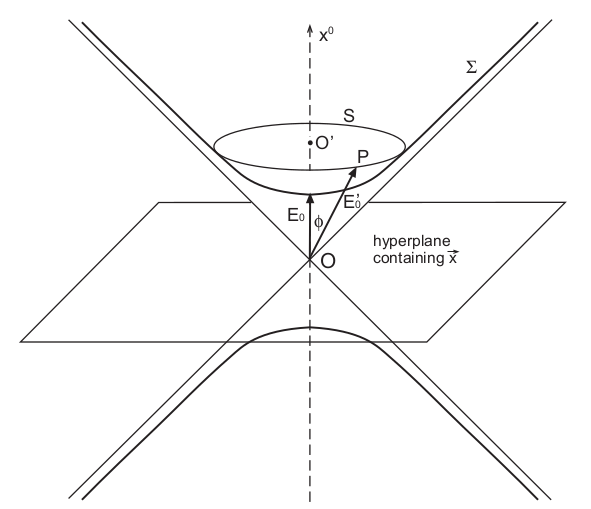
\includegraphics[width=  0.4\linewidth]{hyperboloid_boosts.png}
    \caption[Dominio de la parametrización para las transformaciones de Lorentz puras]{Dominio de la parametrización para las transformaciones de Lorentz puras \footnotemark}
    \label{fig:hiperboloide_boosts}
\end{figure}


El hiperboloide tiene dos ramas dentro del cono de luz, pero si consideramos $x^0>0$ solo necesitamos la primera ($\Sigma$), ya que $L\in\lorentzortopropio$ no puede cambiar el signo de $x^0$. Un \emph{boost} $L:E_0\rightarrow E_0'$ queda unívocamente definido por el punto $P$. Para un $\phi$ dado, $P$ se encuentra en la esfera $S$ (un círculo en la figura \ref{fig:hiperboloide_boosts}) y necesitamos dos parámetros más para fijar la posición de $P$ en $S$. En el espacio de Minkowski $\phi$ se convierte en imaginario, y corresponde a $\psi=i\phi$. \medskip

\footnotetext {Giovanni Costa, Gianluigi Fogli, \emph{Symmetries and Group Theory in Particle Physics} p. 48}


Las propiedades topológicas de este espacio de parámetros nos permiten inferir las siguientes propiedades de $\lorentzortopropio$:
\begin{itemize}
\item $\lorentzortopropio$ es un grupo\textbf{no compacto}, al no ser compacto el hiperboloide.
\item $\lorentzortopropio$ es \textbf{doblemente conexo}. El subconjunto de los \emph{boosts} $L$ es simplemente conexo, puesto que cualquier camino cerrado en $\Sigma$ se puede deformar de forma continua a un punto. Sin embargo, como ya vimos, el subgrupo $\SO$ de las rotaciones es doblemente conexo, y por tanto lo es el propio $\lorentzortopropio$. 
\end{itemize} 

\begin{flushleft}
\textbf{Recubridor universal} de $\lorentzortopropio \cong\mathrm{SO}(1,3)$: grupo simplemente conexo homeomorfo a 
$\lorentzortopropio$. 
\end{flushleft}

Asociamos a cada 4-vector la matriz hermítica
\begin{equation}
X=\sigma_\mu x^\mu =\begin{pmatrix}
x^0+x^3& x^1-ix^2\\
x^1+ix^2&x^0-x^3
\end{pmatrix}\label{matriz_X_Lorentz}
\end{equation}
con $\sigma_\mu:=(\sigma_0,\vec{\sigma}),\qquad\sigma^\mu\equiv \underline{\sigma}_\mu:=(\sigma_0,-\vec{\sigma}),\qquad\sigma_0:=\mathbb{1}_{2\times 2}$. \medskip

% \begin{gather}
% \sigma_\mu:=(\sigma_0,\vec{\sigma})\\
% \sigma^\mu\equiv \underline{\sigma}_\mu:=(\sigma_0,-\vec{\sigma})\\
% \sigma_0:=\mathbb{1}_{2\times 2}
% \end{gather}

Se verifica
\begin{gather}
\trace{\underline{\sigma}_\mu \sigma_\nu}=2\eta_{\mu\nu}\\
x^\mu=\frac{1}{2}\trace{\underline{\sigma}^\mu X}
\end{gather}

% Nótese que $\det X=x\cdot x$

Introducimos una matriz compleja unimodular
\begin{equation}
A=\begin{pmatrix}
\alpha &\beta \\
\gamma &\delta
\end{pmatrix}  \quad \text{con}\quad \det A=\alpha\delta-\beta\gamma=1
\label{matrices_A_Lorentz}
\end{equation}
% con $\det A=1$,
 y transformemos $X$ según
\begin{equation}
X'=AXA^\dagger\Rightarrow x'\cdot x'=\det X'=\det X= x\cdot x
\end{equation}

$A$ describe una transformación lineal de $x^\mu$ que deja $x\cdot x$ invariante, esto es, una transformación de Lorentz. La relación entre matrices $A$ y $\Lambda$ está dada por
\begin{gather}
\Delta^\mu_{\ \nu}\  x^\nu= x'\mu=\frac{1}{2} \trace{\underline{\sigma}^\mu X'}= \frac{1}{2}\trace{\underline{\sigma}^\mu A \sigma_\nu A^\dagger }\ x^\nu \\
\therefore \Lambda^\mu_{\ \nu}= \frac{1}{2}\trace{\underline{\sigma}^\mu A \sigma_\nu A^\dagger }
\end{gather}


El conjunto de matrices $A$ dadas por \eqref{matrices_A_Lorentz} forman el grupo $\mathrm{SL}(2,\mathbb{C})$. Por cada matriz $A$ hay una transformación de Lorentz $\Lambda$, y por cada transformación de Lorentz $\Lambda$ hay dos matrices de $\SL$: $A$ y $-A$. En particular, tanto $\mathbb{1}$ como $-\mathbb{1}$ se corresponden con la identidad en $\lorentzortopropio$. Esta relación entre $\SL$ y $\lorentzortopropio$ es un homomorfismo, ya que preserva la estructura de grupo. \medskip

Podemos escribir $A=e^S$, con $S$ una matriz $2\times 2$ de traza nula. Hay 6 matrices $2\times 2$ sin traza que sean independientes, podemos elegir las 3 matrices de Pauli hermíticas $\sigma_k$ y las tres matrices anti-hermíticas $i\sigma_k$. Entonces, en general, $S=S_1+S_2$ con
\begin{flalign}
&S_1=-i\frac{\phi}{2}\vec{n}\cdot\vec{\sigma}\\
&S_2=-\frac{\psi}{2}\vec{u}\cdot \vec{\sigma}
\end{flalign} 
donde $\phi$ y $\psi$ son parámetros reales y $\vec{n}$ y $\vec{u}$ vectores unitarios reales. \medskip

Obtenemos \underline{dos tipos de matrices: unitarias y hermíticas}.
\begin{flalign}
& U=e^{S_1}=\cos\left(\frac{\phi}{2}\right)\mathbb{1}-i\sin\left(\frac{\phi}{2}\right) \vec{n}\cdot \vec{\sigma}\in \SU\subset\SL\\
&H=e^{S_2}=\cosh \left(\frac{\psi}{2}\right)\mathbb{1}-i\sinh\left(\frac{\psi}{2}\right) \vec{u}\cdot \vec{\sigma}
\end{flalign}
que corresponden a rotaciones puras y a \emph{boosts} puros (con $\vec{\beta}=\vec{u}\tanh \psi$) respectivamente. \medskip

Un teorema de álgebra lineal garantiza que toda matriz $A\in\SL$ se puede escribir como $A=HU$. El homomorfismo entre $\SL$ y $\lorentzortopropio$ implica
\begin{equation}
\Lambda(A)=\Lambda(H)\Lambda(U)\Longrightarrow \boxed{\Lambda=LR}
\end{equation}

\begin{flushleft}
\textbf{Álgebra de Lie} de $\lorentzortopropio$. Como ya sabemos, las transformaciones infinitesimales se corresponden con los generadores del álgebra.
\end{flushleft}
El subgrupo de las rotaciones espaciales puras es generado por tres elementos independientes, que escogemos $R_1(\phi),\ R_2(\phi)$ y $R_3(\phi)$ (vistas como matrices $4\times 4$. 
\begin{equation}
\left(\begin{array}{c|c}
1&\\
\hline
& R_i(\phi)_{3\times3 }
\end{array}\right)
\end{equation}

Los generadores hermíticos de estas rotaciones son
\begin{gather}
J_k=i\left.\parder{R_k}{\phi}\right|_{\phi=0}\qquad k=1,2,3\\
\left(\begin{array}{c|c}
0&\\
\hline
& (J_i)_{\SO}
\end{array}\right)\\
J_{1}=\left(\begin{array}{cccc}{0} & {0} & {0} & {0} \\ {0} & {0} & {0} & {0} \\ {0} & {0} & {0} & {-i} \\ {0} & {0} & {i} & {0}\end{array}\right), \quad J_{2}=\left(\begin{array}{cccc}{0} & {0} & {0} & {0} \\ {0} & {0} & {0} & {i} \\ {0} & {0} & {0} & {0} \\ {0} & {-i} & {0} & {0}\end{array}\right), \quad J_{3}=\left(\begin{array}{cccc}{0} & {0} & {0} & {0} \\ {0} & {0} & {-i} & {0} \\ {0} & {i} & {0} & {0} \\ {0} & {0} & {0} & {0}\end{array}\right)
\end{gather}

Una rotación infinitesimal pura (de ángulo $\delta\phi$) viene dada por
\begin{equation}
R=\mathbb{1}-i\delta\phi\vec{n}\cdot\vec{J}
\end{equation}


Análogamente, podemos derivar los generadores infinitesimales anti-hermíticos $K_l$ de los \emph{boosts} a partir del conjunto linealmente independiente $\{L_1(\psi),L_2(\psi),L_3(\psi)\}$

\begin{gather}
K_l=i\left. \parder{L_l}{\psi}\right|_{\psi=0}\qquad l=1,2,3\\
K_{1}=\left(\begin{array}{cccc}{0} & {-i} & {0} & {0} \\ {-i} & {0} & {0} & {0} \\ {0} & {0} & {0} & {0} \\ {0} & {0} & {0} & {0}\end{array}\right), K_{2}=\left(\begin{array}{cccc}{0} & {0} & {-i} & {0} \\ {0} & {0} & {0} & {0} \\ {-i} & {0} & {0} & {0} \\ {0} & {0} & {0} & {0}\end{array}\right), K_{3}=\left(\begin{array}{cccc}{0} & {0} & {0} & {-i} \\ {0} & {0} & {0} & {0} \\ {0} & {0} & {0} & {0} \\ {-i} & {0} & {0} & {0}\end{array}\right)
\end{gather}

Un \emph{boost} infinitesimal puro (de rapidez $\delta\psi$) a lo largo de la dirección $\vec{n}$ está dado por
\begin{equation}
L=\mathbb{1}-i\delta\psi \vec{u}\cdot \vec{K}\qquad \vec{u}=\frac{\vec{v}}{\abs{\vec{v}}}
\end{equation}

Las transformaciones finitas se obtienen de exponenciar el álgebra\footnote{Aunque formalmente $\Lambda=LR$, la $\Lambda$ dada por \eqref{Lorentz_general_finita} NO es el producto de la $L$ dada por \eqref{boost_finito} por la $R$ dada por \eqref{rotacion_finita}.}
\begin{flalign}
&R=e^{-i\phi \vec{n}\cdot \vec{J}} \label{rotacion_finita}\\
&L=e^{-i\psi \vec{u}\cdot \vec{K}} \label{boost_finito}\\
&\Lambda= e^{-i(\phi \vec{n}\cdot \vec{J}+\psi \vec{u}\cdot \vec{K})} \label{Lorentz_general_finita}
\end{flalign}

El álgebra de Lie de $\lorentzortopropio$ y dde $\SL$ cumple las  \textbf{reglas de conmutación} siguientes
\begin{subequations}
\begin{flalign}
\left[J_{i}, J_{j}\right] &=i \epsilon_{i j k} J_{k} \\\left[K_{i}, K_{j}\right] &= - i \epsilon_{i j k} J_{k} \\\left[J_{i}, K_{j}\right] &=i \epsilon_{i j k} K_{k} 
\end{flalign}
\label{conmutadores_lorentz}
\end{subequations}

Definimos el tensor antisimétrico $M_{\mu\nu}$ de componentes
\begin{flalign}
&\left(M_{12}, M_{23}, M_{31}\right)=\left(J_{3}, J_{1}, J_{2}\right) \longrightarrow M_{ij}=\epsilon_{ijk}J_k\\ 
&\left(M_{01}, M_{02}, M_{03}\right)=\left(K_{1}, K_{2}, K_{3}\right)\longrightarrow M_{0i}=K_i=-M_{i0}
\end{flalign}

de modo que los conmutadores \eqref{conmutadores_lorentz} en forma covariante resultan
\begin{equation}
\left[M_{\lambda \rho}, M_{\mu \nu}\right]=-i\left(\eta_{\lambda \mu} M_{\rho \nu}+\eta_{\rho \nu} M_{\lambda \mu}-\eta_{\lambda \nu} M_{\rho \mu}-\eta_{\rho \mu} M_{\lambda \nu}\right)
\end{equation}
y una transformación general de $\lorentzortopropio{}$ se puede escribir como
\begin{equation}
\Lambda=e^{-\frac{1}{2} i \omega^{\mu \nu} M_{\mu \nu}}
\end{equation}
donde $\omega^{\mu\nu}$ es una matriz real antisimétrica. \medskip

Se tienen los dos \textbf{Casimires}
\begin{flalign}
 \frac{1}{2} M^{\mu \nu} M_{\mu \nu} &=\vec{J}^{2}-\vec{K}^{2} \\ 
 \frac{1}{2} \epsilon^{\mu \nu \sigma \tau} M_{\mu \nu} M_{\sigma \tau} &=-\vec{J} \cdot \vec{K} 
\end{flalign}


\begin{flushleft}
\textbf{Representaciones irreducibles de} $\lorentzortopropio\cong\mathrm{SO}(1,3)$. Al ser $\lorentzortopropio$ no compacto, dichas representaciones no pueden ser unitarias. Al no ser hermíticos los generadores $\vec{K}$, las matrices $\Lambda$ en general no serán unitarias.
\end{flushleft}

Para clasificar las representaciones irreducibles introducimos las siguientes combinaciones de generadores
\begin{subequations}
\begin{flalign}
M_{i}=\frac{1}{2}\left(J_{i}+i K_{i}\right)\\
N_{i}=\frac{1}{2}\left(J_{i}-i K_{i}\right)
\end{flalign}
\end{subequations}
 que son hermíticas. Cumplen las reglas de conmutación
\begin{flalign}
&\left[M_{i}, M_{j}\right]=i \epsilon_{i j k} M_{k}\\
&\left[N_{i}, N_{j}\right]=i \epsilon_{i j k} N_{k}\\
&\left[M_{i}, N_{j}\right]=0
\end{flalign}

$\vec{M}$ y $\vec{N}$ son los generadores de dos copias de $\su_{\mathbb{C}}$ ($\su$ complejificado). Es decir, si denotamos por $M_{\mathbb{C}}$ y $N_{\mathbb{C}}$ la envolvente lineal compleja de $\vec{M}$ y $\vec{N}$ tenemos el isomorfismo
\begin{equation}
\mathfrak{so}(1,3)_{\mathbb{C}}=M_{\mathbb{C}}\ \oplus\ N_{\mathbb{C}}\cong \su_{\mathbb{C}}\ \oplus\ \su_{\mathbb{C}}\cong \mathfrak{sl}(2,\mathbb{C})\ \oplus\ \mathfrak{sl}(2,\mathbb{C})
\end{equation}

Tenemos que
\begin{subequations}
\begin{flalign}
&[\vec{M}^2,M_i]=0\\
&[\vec{N}^2,N_i]=0
\end{flalign}
\end{subequations}
por lo que podemos etiquetar las representaciones irreducibles de $\lorentzortopropio$ con los autovalores $j(j+1)$ y $j'(j'+1)$ de los Casimir $\vec{M}^2$ y $\vec{N}^2$ respectivamente, donde $j,j'=0,1/2,1,3/2,\ldots$\medskip


 Podemos tomar los $d=(2j+1)(2j'+1)$ autoestados independientes como base del EV sobre el que actúa la representación irreducible de dimensión $d$ de $\lorentzortopropio$. Cada elemento $\Lambda\in\lorentzortopropio$ queda representado por una matriz $D^{(j,j')}(\Lambda)$. \bigskip

Restringiéndonos al subgrupo de rotaciones $\SO$, las representaciones dejan de ser irreducibles y pueden descomponerse en términos de las representaciones irreducibles de $\SO$ de la forma

\begin{equation}
D^{\left(j, j^{\prime}\right)}(R)=D^{(j)}(R) \otimes D^{\left(j^{\prime}\right)}(R)=D^{\left(j+j^{\prime}\right)}(R) \oplus \ldots \oplus D^{\left(\left|j-j^{\prime}\right|\right)}(R)
\end{equation}

Al igual que para $\SO$ se tienen dos clases de representaciones irreducibles para $\lorentzortopropio$: tensoriales y espinoriales, con $j+j'$ entero y semi-entero respectivamente. Las espinoriales se obtienen de su recubridor universal $\SL$ y desde el punto de vista de $\lorentzortopropio$ son bivaluadas --al ser $\lorentzortopropio$ doblemente conexo, sus elementos admiten dos representaciones de $\SL$. Mientras que los campos tensoriales se transforman bien  bajo $\mathrm{SO}(1,3)$, los campos espinoriales se transforman bajo $\SL$, análogamente a los tensores y espinores de $\SO$ y $\SU$.

\begin{flushleft}
\textbf{Representaciones de espín más bajo}. Hay dos representaciones de dimensión 2 inequivalentes: $D^{(\frac{1}{2},0)}$ y $D^{(0,\frac{1}{2})}$
\end{flushleft}

Mientras que $\Lambda(A)=\Lambda(-A)$, $A$ y $\bar{A}$ no dan lugar a representaciones equivalentes. Como en general las matrices $A\in \SL$ no son unitarias, no hay una transformación de similaridad que relacione $A$ con $\bar{A}$. En el caso de las rotaciones, una representación y su compleja conjugada sí que son equivalentes.\medskip

Las matrices $A$ y $\bar{A}$ constituyen, en general, dos representaciones irreducibles inequivalentes de $\lorentzortopropio$ que actúan en dos espacios vectoriales diferentes. Tenemos entonces dos bases no equivalentes y, generalmente, dos clases de biespinores (contravariantes): $\xi$ y $\overline{\xi}$.\medskip

Estos biespinores se transforman de acuerdo a 

\begin{subequations}
\begin{flalign}
&\xi'=A\xi \qquad \text{en comps. contravariantes:  } \xi= \begin{pmatrix}
\xi^1 \\ \xi^2
\end{pmatrix}\quad \xi^{\prime\alpha}=A^\alpha_{\ \beta} \xi^\beta\quad \alpha,\beta=1,2\\
&\bar{\xi}'=\bar{A}\bar{\xi} \qquad \text{en comps. contravariantes:  } \bar{\xi}= \begin{pmatrix}
\xi^{\dot{1}} \\ \xi^{\dot{2}}
\end{pmatrix}\quad  \bar{\xi}^{\prime\dot{\alpha}}=\bar{A}{\dot{\alpha}}_{\ \dot{\beta}} \xi^{\dot{\beta}}\quad \alpha,\beta=1,2
\end{flalign}
\end{subequations}

En términos de componentes covariantes $\eta=\left(\eta_{1} \quad \eta_{2}\right), \bar{\eta}=\left(\eta_{\mathrm{i}} \quad \eta_{\dot{2}}\right)$
\begin{subequations}
\begin{flalign}
&\eta_{\alpha}^{\prime}=\eta_{\beta}\left(A^{-1}\right)_{\alpha}^{\beta} \Longleftrightarrow \eta'=\eta A^{-1}\\
&\eta_{\dot{\alpha}}^{\prime}=\eta_{\dot{\beta}}\left(\bar{A}^{-1}\right)_{\dot{\alpha}}^{\dot{\beta}}\Longleftrightarrow \bar{\eta}'=\bar{\eta}A^\dagger
\end{flalign}
\end{subequations}
y los productos $\eta\xi$ y $\bar{\eta} \bar{\xi}$ son invariantes (escalares bajo $\lorentzortopropio$). \medskip


Queremos obtener los generadores $\vec{J}$ y $\vec{K}$ para las representaciones $A$ y $\bar{A}$. Sabemos que 
\begin{gather}
A=e^{-\frac{i}{2}(\phi \vec{n}\cdot \vec{\sigma}-i\psi \vec{u}\cdot\vec{\sigma})}\\
A=e^{-\frac{i}{2}(-\phi \vec{n}\cdot \vec{\sigma}^*-i\psi \vec{u}\cdot\vec{\sigma}^*)}\\
D=e^{-i(\phi \vec{n}\cdot \vec{J}+\psi \vec{u}\cdot \vec{K})}
\end{gather}
de modo que
\begin{itemize}
\item Para los espinores $\xi\quad J_i=\frac{1}{2}\sigma_i,\ K_i=-\frac{i}{2}\sigma_i\Longrightarrow M_i=\frac{\sigma_i}{2},\enskip N_i=0\leadsto j=\frac{1}{2},\enskip j'=0\longrightarrow D^{\left(\frac{1}{2},0\right)}(\Lambda)$
\item Para los espinores $\bar{\xi}\quad J_i=-\frac{1}{2}\sigma_i,\ K_i=-\frac{i}{2}\sigma_i$. Como $\sigma_2\sigma_i^*\sigma_2=-\sigma_i$, esta representación es equivalente a $S_i=\frac{1}{2}\sigma_i,\enskip K_i=\frac{i}{2}\sigma_i\Longrightarrow M_i=0,\enskip N_i=\frac{\sigma_i}{2}\leadsto j=0,\enskip j'=\frac{1}{2}\longrightarrow D^{\left(0,\frac{1}{2}\right)}(\Lambda)$
\end{itemize}

$A$ y $(A^t)^{-1}$ están relacionadas por una transformación de similaridad, de modo que corresponden a representaciones equivalentes:
\begin{equation}
\exists C\in\SL \text{ tal que } (A^t)^{-1}=CAC^{-1}\Leftrightarrow C=A^tCA 
\end{equation}

En particular, para $C=i\sigma_2$ se tiene
\begin{equation}
\tilde{\eta}^{\prime}=\tilde{A}^{-1} \tilde{\eta}=C A C^{-1} \tilde{\eta}\Longrightarrow\tilde{\eta}=C \xi
\end{equation}

\begin{flushleft}
\textbf{Representación de dimensión 4: $D^{\left(\frac{1}{2},\frac{1}{2}\right)}$}. El EV es el de los 4-vectores $x^\mu$ que se transforman de acuerdo con \eqref{transf_coords_4_vector} o \eqref{matriz_X_Lorentz}. Consideremos la cantidad $\xi\bar{\xi}$ que se transforma según
\end{flushleft}
\begin{equation}
\xi'\xi^{\prime\dagger} =A\xi\xi^\dagger A^\dagger
\end{equation}
al igual que $X'$. \medskip

Es decir que podemos tomar $\xi\xi^\dagger$ como la base del espacio de representación $D^{\left(\frac{1}{2},\frac{1}{2}\right)}$. Esto es consistente con
\begin{equation}
D^{\left(\frac{1}{2},\frac{1}{2}\right)}=\underbrace{D^{\left(\frac{1}{2},0\right)}}_\xi \otimes \underbrace{D^{\left(0,\frac{1}{2}\right)}}_{\bar{\xi}}
\end{equation}
y por tanto debe contener los dos tipos de espinores $\xi$ y $\bar{\xi}$.


\begin{nota}
Si queremos mantener la correspondencia entre representaciones irreducibles y estados de espín bien definido para $\lorentzortopropio$ (al igual que para $\SO$) tenemos que introducir condiciones extra que reduzcan el número de elementos independientes de la base. En particular, una partícula de espín 1 se describe con una base de 4 dimensiones, por lo que necesitamos una condición extra para dejar solo 3 elementos independientes, llamada condición de Lorentz:
\begin{equation}
\partial_\mu A^\mu (x)=0
\end{equation}
(para fotones).
\end{nota} 


\begin{flushleft}
\textbf{Transformación de funciones escalares.} El espacio de funciones $\psi(x)$ con $x=(x^0,x^i)=(ct,-x_i)$ proporciona una representación de los operadores $X_\mu,\ P_\mu$ y $M_{\mu\nu}$:
\end{flushleft}
\begin{flalign}
&X_\mu \psi(x)=x_\mu \psi(x)\\
&P_\mu \psi(x)=\textcolor{red} {+} i\partial_\mu \psi(x) \label{momento_lorentz}\\
& M_{\mu\nu}=X_{\mu}P_{\nu} -X_{\nu}P_{\mu}
\end{flalign}
donde el signo positivo en \eqref{momento_lorentz} proviene de la signatura $(+,-,-,-)$.\medskip

Para una transformación de Lorentz infinitesimal
\begin{flalign}
 \delta x^\mu &=x^{\prime\mu}-x^\mu=-\frac{i}{2} \delta\omega^{\rho\sigma} (M_{\rho\sigma})^\mu_{\ \nu}\ x^\nu\\
 \delta \psi(x)&=\psi'(x)-\psi(x)=\psi'(x'-\delta x)-\psi(x)=-\delta x^\mu \partial_\mu \psi(x)\nonumber \\
 &=\frac{i}{2} \delta\omega^{\rho\sigma} (M_{\rho\sigma})^\mu_{\ \nu}\ x^\nu\parder{}{x^\mu} \psi(x)\equiv -\frac{i}{2} \delta\omega^{\rho\sigma} \tilde{M}_{\rho\sigma}(\psi)
\end{flalign}
con
\begin{flalign}
&(M_{\rho\sigma})^\mu_{\ \nu}=i\left(\eta_{\rho}^{\ \mu}\eta_{\sigma\nu} - \eta_{\sigma}^{\ \mu}\eta_{\rho\nu}\right)\\
&\tilde{M}_{\rho\sigma}=-i\left(\eta_{\rho}^{\ \mu}\eta_{\sigma\nu} - \eta_{\sigma}^{\ \mu}\eta_{\rho\nu}\right)x^\nu \parder{}{x^\mu}=-i \left(x_\sigma \parder{}{x^\rho}-x_\rho \parder{}{x^\sigma} \right)= X_\rho P_\sigma -X_\sigma P_\rho
\end{flalign}

\newpage
\begin{flushleft}
\textbf{Espinor de Weyl levógiro.} Campo $\psi_L(x)$ que bajo $\Lambda$ se transforma en la representación $\left(\frac{1}{2},0\right)$, es decir se transforma según
\end{flushleft}
\begin{equation}
\psi_L(x)\xrightarrow{\Lambda}  \psi_L'(x')=\underbrace{e^{(-i\phi \vec{n}-\psi \vec{u})\cdot \frac{\vec{\sigma}}{2}}  }_{\Lambda_L}\ \psi_L(x)
\end{equation}
con
\begin{equation}
\Lambda_L=e^{(-i\phi \vec{n}-\psi \vec{u})\cdot \frac{\vec{\sigma}}{2}}   \label{lambda_Weyl_A}
\end{equation}

Veamos la representación de los generadores de Lorentz sobre $\psi_L$
\begin{flalign}
\delta \psi_L(x)&=\psi_L'(x)-\psi_L(x)=\psi_L'(x'-\delta x)-\psi_L(x)=\nonumber \\
&=\underbrace{\psi'_L(x')}_{\Lambda_L\psi_L(x)}-\delta x^\mu \parder{}{x^\mu} \psi(x)-\psi_L(x)=(\Lambda_L-\Lambda)\psi_L(x)-\delta x^\mu \parder{}{x^\mu} \psi(x)
\end{flalign}

Escribiendo $\Lambda_L$ de la forma
\begin{equation}
\Lambda_L=e^{-\frac{i}{2}\delta \omega^{\mu\nu}\tilde{S}_{\mu\nu}}=1-\frac{i}{2}\delta \omega^{\mu\nu}\tilde{S}_{\mu\nu} \label{lambda_Weyl_B}
\end{equation}
se tiene
\begin{equation}
\delta \psi_L=-\frac{i}{2}\delta \omega^{\mu\nu}\tilde{J}_{\mu\nu}\psi_L
\end{equation}
con $\tilde{J}_{\mu\nu}$ el momento angular total:
\begin{equation}
\tilde{J}_{\mu\nu}=\tilde{M}_{\mu\nu}+\tilde{S}_{\mu\nu}
\end{equation}
donde $\tilde{M}_{\mu\nu}$ aparece siempre y $\tilde{S}_{\mu\nu}$ depende de la representación.\medskip

Comparando las dos  expresiones para $\Lambda_L$, \eqref{lambda_Weyl_A} y \eqref{lambda_Weyl_B}, deducimos
\begin{subequations}
\begin{flalign}
&S_i=\frac{1}{2}\epsilon_i^{\ jk} S_{jk}=\frac{\sigma_i}{2}\\
&S_{0i}=-i\frac{\sigma_i}{2}
\end{flalign}
\end{subequations}
de modo que $j=\frac{1}{2}$ y $j'=0$. \underline{Los espinores de Weyl se transforman en la representación $D^{\left(\frac{1}{2},0\right)}$}.\medskip

Análogamente, los espinores de Dirac se transforman en la representación $D^{\left(\frac{1}{2},\frac{1}{2}\right)}$.

\end{document}

